\chapter{Evaluation}\label{ch:evaluation}

% Second most important chapter. Verifies the theses defined in the previous chapter.
% Tries to evaluate and analyze the contribution in qualitative or quantitative terms.
% Ends with a discussion. Approximately 10 to 15 pages. Can be split into multiple chapters.

To begin with, we introduce the \acs*{rouge} metrics we use during evaluation
and briefly explain how these values can be interpreted in \autoref{sec:rouge}.
Afterward, we present the three datasets used in this work,
explain how we select training and test data,
and compare them with summarization datasets from other domains in \autoref{sec:datasets}.

Then we report on the concrete experiments conducted:
First evaluating a preliminary experiment to determine suitable separators between log messages (\autoref{sec:preliminary_separators}),
second, an extensive evaluation of different summarization models (\autoref{sec:evaluation_experiment_finetuned}),
followed by an experiment to explore the effects of further pre-training on log-data (\autoref{sec:evaluation_experiment_pretraining}).
Finally, we present a direct comparison of the best-performing model with a previous log summarization framework (\autoref{sec:evaluation_experiment_logsummary}).

At the end of this chapter, we discuss potential threats to validity we see with our work in \autoref{sec:threats_to_validity}.

\section{Using the \acs*{rouge} Metric for Evaluation}\label{sec:rouge}

In the previous chapter we introduced several models and the tasks we evaluate them on,
yet the question remains how to judge the performance of our models.
As abstractive \ac{seq2seq} models produce arbitrary text,
one cannot directly determine a set of \emph{true} and \emph{false} predictions,
to measure accuracy for instance.

Deciding whether a text is a good summary of another text is not a straightforward, objective question.
Rather we have to rely on metrics such as the widely used collection of \acs*{rouge}-metrics~\parencite{rouge},
which has become a de facto standard for judging the performance of summarization models.%
\footnote{See for example the benchmarks on \url{https://paperswithcode.com/task/text-summarization}.}

Originally, \ac{rouge} was introduced to provide a set of metrics to judge the quality of a summary automatically.
This is achieved by comparing it to other reference summaries usually created by humans~\parencite[74]{rouge}.

As such, it analyzes so-called \(n\)-grams between
a \emph{reference} text and a \emph{candidate} text that is to be evaluated,
and defines different metrics based on their matching \(n\)-grams.
In the context of \acl{nlp} pairs of words are usually referred to as bigrams~\parencite[30-31]{statistical_nlp};
consequently, \(n\)-grams are the generalization of this concept and simply refer to a sequence of \(n\) words or tokens.

We use a port of the original implementation provided by the Google Research Team.%
\footnote{The repository is available at: \url{https://github.com/google-research/google-research/tree/9f5bedb711b322125505336fac58ef6261911ca4/rouge}}
Here, unigrams (\(n\)-grams with \(n = 1\)) are determined as continuous sequences of non-alphanumerical characters,
which are then lowercased.
\(n\)-grams are computed as sequences of these unigrams.
Consequently, the metric analyzes the whole text at once and ignores sentence boundaries indicated by punctuation.
Contrary to the original, Google's implementation does not support \emph{stopword removal},
that is the removal of words that play an important role in the construction of English sentences,
but are less likely to contribute important information~\parencite[533-534]{statistical_nlp}.
% \textcquote[533-534]{statistical_nlp}{words \textins{that} have important semantic functions in English,
% but \textelp{} rarely contribute information \textelp{in} a simple word-by-word match}.
Common examples for stop words are \emph{the}, \emph{from} or \emph{could}~\parencite[533]{statistical_nlp}.

In the following segments, we intend to explain the two families of \acs*{rouge}-metrics
we use for evaluation in our experiments.
Although \acs*{rouge} was designed to be able to compare a candidate summary to multiple reference summaries,
we will only ever have a single reference summary to compare to,
hence why we will not explain how to apply \acs*{rouge} with multiple references.

\paragraph{\acs*{rouge}-\(n\)}
\newcommand{\matchcount}{\ensuremath{\#\texttt{match}}}
Vital to the computation of \acs*{rouge}-\(n\) is the number of \(n\)-grams occurring both in the candidate and reference summary~\parencite[1]{rouge},
which we will refer to as \(\matchcount\).
Given the sequence of n-grams in the candidate text \(C_n\) and reference text \(R_n\),
as well as a function \(\#_X(t)\)
counting the occurrences of an element \(t\) in a sequence \(X\),
we can determine \(\matchcount\) to be
\begin{equation}
\matchcount(C_n, R_n) = \sum_{t \,\in\, C_n \cup\, R_n} \min(\#_{C_n}\!(t), \#_{R_n}\!(t))
\end{equation}
where \(X \cup Y\) is the set-union of two sequences \(X\) and \(Y\)
(\(X, Y\) are each transformed each into a set of their unique sequence elements,
then the union of the resulting two sets is taken).

The \acs*{rouge}-\(n\) recall is then defined as
\begin{equation}
\text{\acs*{rouge}-}n_\text{recall} = \frac{\matchcount(C_n, R_n)}{|R_n|}
\end{equation}
where \(|X|\) refers to the length of a sequence \(X\).
Depending on the choice of \(n\) one gets different results;
\acs*{rouge}-1 measures the overlap in words between reference and candidate summaries (\(n = 1\)),
\acs*{rouge}-2 measures the overlap of word-pairs (\(n = 2\)), and so forth.

In \parencite{rouge}, only the \acs*{rouge}-\(n\) recall metric is mentioned,
but we are equally interested in the precision and \(F_1\)-measure of \acs*{rouge}-\(n\),
which were added in a later version of ROUGE.%
\footnote{A copy of the updated implementation can be found at \url{https://github.com/andersjo/pyrouge/tree/3b6c415204dbc2c8360a01d92533441f4aae95eb/tools/ROUGE-1.5.5};
originally the script would be sent via email, as explained on its nowadays unreachable website \url{https://web.archive.org/web/20161205014058/http://www.berouge.com/Pages/default.aspx}.}

The \acs*{rouge}-\(n\) precision is defined as
\begin{equation}
\text{\acs*{rouge}-}n_\text{precision} = \frac{\matchcount(C_n, R_n)}{|C_n|}
\end{equation}
%
Suppose we understand the overlap in \(n\)-grams as an approximation of the information a reference and candidate summary have in common
and declare only the information contained in a reference summary as \enquote{important}.
In that case, \acs*{rouge}-\(n\) recall tells us how much of the important information is contained in a candidate summary,
while precision measures what ratio of a candidate summary is important.

Intuitively, a good summary usually contains a lot of the important information (\emph{recall})
but is also to the point and does not contain much unnecessary information (\emph{precision}).
However, it would be beneficial to compare the recall and precision in a single, combined metric to get a final indicator of a summary's quality.
To this end, we can employ the \(F_1\)-measure, which is the harmonic mean of recall and precision:
\begin{equation}
F_1 = 2 \cdot \frac{\text{recall} \cdot \text{precision}}{\text{recall} + \text{precision}}
\end{equation}
% \begin{equation}
% \text{\acs*{rouge}-}n_\text{F_1} = 2 \cdot \frac{\text{\acs*{rouge}-}n_\text{recall} \cdot \text{\acs*{rouge}-}n_\text{precision}}{\text{\acs*{rouge}-}n_\text{recall} + \text{\acs*{rouge}-}n_\text{precision}}
% \end{equation}
%
Going forward, we will imply the use of the \(F_1\)-measure for \acs*{rouge}-\(n\)
when we refer to \emph{\acs*{rouge}-\(n\) scores} unless stated otherwise.\\
When reporting \acs*{rouge}-scores, we report them in percent, but omit the percent sign,
e.g. a \acs*{rouge}-1 recall of \(0.245\) is reported as a \acs*{rouge}-1 recall-score of \(24.5\).
This also applies to any \acs*{rouge}-L scores we mention, which we explain in the next segment.

\paragraph{\acs*{rouge}-L}
\newcommand{\lcs}{\ensuremath{\texttt{LCS}}}
Essential to \acs*{rouge}-L is the concept of the \emph{longest common subsequence} \(\lcs\).
Given a sequence \(X = (x_0, x_1, \ldots, x_n)\) we can write any arbitrary subsequence of \(X\) as
\(Z = (x_{i_0}, x_{i_1}, \ldots, x_{i_j})\) with \(0 <= i_0 < i_1 < \ldots < i_j <= n\).
Such a subsequence \(Z\) may contain less elements than \(X\) but preserves the order of elements.

The longest common subsequence \(\lcs(X, Y)\) of two sequences \(X, Y\) is the longest sequence \(Z\) that is both a subsequence of \(X\) and \(Y\).
Intuitively, if two sentences share a long common subsequence, they not only contain similar information
but also follow related sentence structures~\parencite[3]{rouge}.
\acs*{rouge}-L normalizes the \(\lcs\) to the lengths of the texts that are compared.

Given the sequence of words (\emph{unigrams}) in the candidate text \(C_1\) and reference text \(R_1\),
as well as the function \(\lcs(X, Y)\) which determines the longest common subsequence of the sequences \(X\) and \(Y\),
\emph{sentence-level} \acs*{rouge}-L recall and precision are defined as follows:
\begin{align}
\text{\acs*{rouge}-LSent}_\text{recall}    &= \frac{\lcs(C_1, R_1)}{|R_1|}\\
\text{\acs*{rouge}-LSent}_\text{precision} &= \frac{\lcs(C_1, R_1)}{|C_1|}
\end{align}
%
\acs*{rouge}-L makes the distinction between sentences and summaries
and uses a different method to determine recall and precision at \emph{summary-level}
with the help of user-provided sentence boundaries.
At the summary-level so-called \emph{union \(\lcs\)} is used~\parencite[3]{rouge}:
The \(\lcs\) is calculated between a sentence in a reference summary
and each sentence of the candidate summary,
and the elements of all individual subsequences are merged to obtain the largest sequence,
that is still a subsequence of the reference summary.
% Given a reference summary consistent of \(m\) sentences (sequences of unigrams)
% \(\mathcal{R} = (R_1^0, R_1^1, \ldots, R_1^m)\)
% and a candidate summary concistent of \(k\) sentences
% \(\mathcal{C} = (C_1^0, C_1^1, \ldots, C_1^k)\),
% \emph{summary-level} \acs*{rouge}-L recall and precision are defined as follows:
% \begin{align}
% \text{\acs*{rouge}-L}_\text{recall}    &= \frac{\sum_{i = 0}^m \lcs_\cup(\mathcal{C}, R_1^i)}{\sum_{i = 0}^m |R_1^i|}\\
% \text{\acs*{rouge}-L}_\text{precision} &= \frac{\sum_{i = 0}^m \lcs_\cup(\mathcal{C}, R_1^i)}{\sum_{i = 0}^k |C_1^i|}
% \end{align}

Thus the information contained in a single reference sentence may be spread
across the whole candidate summary without impacting the overall summary-level score.
Summary-level \acs*{rouge}-L allows the candidate summary to be structured differently from the reference
and is indifferent to the number of sentences a candidate summary has.

% The \acs*{rouge}-L F1-score will always be less or equal to the \acs*{rouge}-1 F1-score~\parencite[2-3]{rouge},
% while the summary-level \acs*{rouge}-L will always be at least as high as at the sentence-level,
% when applyed for the whole summary (ignoring sentence boundaries).

\parencite{rouge} initially proposes a weighted \(F\)-measure to combine \acs*{rouge}-L recall and precision,
which is a generalization of the \(F_1\)-measure,
but the most recent official implementation uses a \(F_1\)-measure by default.\\
As such we also use the \(F_1\)-measure implicitly,
when we refer to \emph{\acs*{rouge}-L scores} unless stated otherwise.

\section{Datasets}\label{sec:datasets}

In principle, any dataset containing logs that adhere to the characteristics laid out in \autoref{sec:summarization_tasks} could be used.
The key property for summarization based on \emph{common log events} to be applicable,
is the existance of multiple logs which can be grouped by root cause.
That way it is possible to extract log-entries corresponding to common log events,
which are the base for any reference summaries.\\
Meanwhile, summarization based on \emph{non-normal log events} can in principle be applied,
if logs have been labeled as abnormal or not.

In the following paragraphs we present the datasets we use individually.

\paragraph{\telco{}}

A global telecommunication and cloud provider has granted us access
to a collection of logs that we will refer to as the \telco{}-dataset.
The logs arise from application crash reports when using enterprise software in a small distributed system,
producing entries of heterogeneous formatting, content, and purpose.
System experts have manually conducted a root cause analysis and grouped the logs by root cause.
For each root cause, there are multiple scenarios from different system failures.
Therefore this dataset is particularly suitable for the summarization based on \emph{common log events}.

% NOTE: Unused.
% Additionally system experts have provided us with a short description of each root cause.
% These descriptions are highly abstractive,
% summarizing entire scenarios containing hundreds of thousands of log-lines in one or two sentences,
% and include knowledge about the system and its (desired) behavior.\\
% Unfortunately the scenarios and descriptions provided are not numerous
% enough to create a log summarization dataset for training an abstractive model.

Since logs in the \telco{}-dataset are very fine-grained,
containing tens of thousands of log-entries for each minute of runtime,
the relevant portions of the logs have to be determined.
To this end, we are also provided with the timestamp of the failure,
but its temporal resolution is too low,
still potentially leaving us with thousands of log-entries.

To further delimit the relevant parts of the logs, we inspect the common log events in a time span around the failure.
For some root causes, we manually determined anomalous log events for which we suspect they represent error events leading up to the failure.
There may be multiple such events per log file.\\
Finally, we extract all entries around these log events using a manually defined
threshold and use these log messages as the baseline for our summarization dataset.
All in all, we gather log-data from two related root causes.

\paragraph{\hadoop{}}

First described by \citeauthor*{hadoop_dataset},
the \hadoop{}-dataset contains logs produced by the Hadoop platform%
\footnote{see \url{https://hadoop.apache.org/}} when running two different applications (PageRank, WordCount) on a cluster spanning multiple computers.
During the execution of each application, failures are provoked manually (machine shutdown, network disconnection, full disk),
thus creating multiple scenarios with the same failures~\parencite[106]{hadoop_dataset}.
There are also several logs available from running the two applications during normal execution, in the absence of any failures.\\
This makes the \hadoop{}-dataset particularly suitable for our summarization task based on \emph{non-normal log events}.

Interestingly, summarization based on \emph{common log events} is not applicable here, even though each log is categorized by failure type:
The common log events between each failure type are almost the same;
there are only a handful of log events common between all logs where a network disconnection occurred,
which do not also occur when the disk is full.
Therefore the common log events do not represent events specific to that failure
but rather to any execution environment;
the common log events are quite dull and represent startup operations, progress indicators and other generic activity.
However basing the summarization on non-normal log events, we can get a concise summary of the failure from each log.

The dataset also features a multitude of short logs from other nodes running in parallel with the node that experienced the failure;
Often a node simply starts up, performs its task successfully and shuts down again.
In these cases no events of interest occur, so we would end up with many empty summaries.
To avoid this situation we choose to exclude any logs with fewer than 200 log-entries from the summarization task.

This method of manually triggering failures used in \parencite{hadoop_dataset} may be well suited to further construct datasets for log summarization.
However going forward we will not explore the creation of more log summarization datasets and instead employ existing datasets for training and evaluation.
As such we will leverage the publicly accessible \hadoop{}-dataset
provided in the context of Loghub~\parencite{loghub} available at \parencite{loghub_datasets}.

\paragraph{\logsummary{}}

Unlike the previous two datasets, the \logsummary{}-dataset is not constructed by us using one of our summarization tasks
but instead contains manually written summaries by \citeauthor*{log_summary} using various datasets from \parencite{loghub_datasets},
originating from various distributed systems, supercomputers, and standalone applications~\parencite{loghub}.

They summarized 601 examples of 20 consecutive log messages selected uniformly from 6 datasets (not including \hadoop{})~\parencite[6]{log_summary}.
2 of these datasets were not reported upon in the original paper, but the summaries are available in their repository.%
\footnote{\url{https://github.com/WeibinMeng/LogSummary/tree/469b1e25f4f759c0ace1c91e2513a4be08831ea7/data/summary/logs}}
All in all, we call this collection of documents and summaries from all 6 (sub-)datasets \emph{the} \logsummary{}-dataset.

Contrary to the previous two datasets we examine,
summaries are not based on the presence of failures,
and input data may represent normal system activity.
On \telco{} and \hadoop{} we would not produce a summary in such cases.
Here we are given summaries of the most relevant contents, even for log-data that can be expected to occur during normal operation.
This makes the task of summarization on this dataset different from the failure-centric summarization on the other two datasets.

Although the summaries are human-written, they still are purely extractive:
Segments deemed most important by the authors are copied from the log entries
and are collected into each summary.

Compared to our other log datasets, \logsummary{}'s documents and summaries are quite short as can be seen in \autoref{tab:other_domains_vs_log_datasets},
and summaries contain only parts of a log message as opposed to being a sequence of entire log messages.

\subsection{Selection of Training and Evaluation Data}\label{subsec:training_test_split}

As pointed out by \citeauthor*{statistical_nlp},
evaluating a model on the same data as the one it was trained on is bad practice:
The evaluation is only fair, if the model is asked to make predictions using data it has not seen before.
Otherwise, a model can simply reconstruct the outputs it has observed during training,
favoring \emph{overfitted} models that did not actually learn to perform the desired task in a more general setting~\parencite[74-75]{statistical_nlp}.

It is common practice to select a only small percentage of a dataset as test data to evaluate on~\parencite{statistical_nlp}.
This would result in too few test examples to draw empirically sound conclusions
because our datasets do not contain many examples.
Furthermore, summaries in our datasets are not very varied,
which is to be expected considering one of our summarization tasks is based on log events \emph{common} between all logs of the same root cause.

Instead, we decide to select a few representative examples for each dataset to train on and evaluate on the overwhelming remainder:
\begin{description}
\item[\logsummary] We randomly select 5 examples from each sub-dataset for a total of 30 training examples and 571 examples for evaluation.
\item[\hadoop] We manually choose representative examples from each application and failure type;
      Per application 5 for the \emph{disk full}-failure and 10 for the \emph{machine shutdown} and
      \emph{network disconnection}-failures resulting in 50 training examples and 1055 examples for evaluation.
\item[\telco] We choose all chunks belonging to one of two log files,
      which leads to 16 training examples and 89 examples for evaluation.
\end{description}
As a practical use case for manual selection of training examples
like on \hadoop{} and \telco{}, we envision the following:
An operator has identified log-data corresponding to an error or set of errors
which may occur repeatedly during system operation,
and would like to speed up any future analyses conducted on such failures or similar ones.
Thus he trains an \emph{expert model} which is able to summarize such log-data
but may fail on more distinct logs.

To judge the representativeness and diversity of our training and test sets,
we calculate the overlap in the vocabulary of words used in the summaries between the training and test sets,
shown in \autoref{tab:training_test_vocab_overlap}.
For comparison, we also include this ratio for the commonly used training and test splits
on the XSum news article summarization dataset.
As was to be expected, the overlap on the \telco{}-dataset is large,
as we use the common log events between the logs as summaries.
On the other two datasets, our training examples contain a large part of the words used in test data,
which speak for their representativeness.
Nonetheless, there are still some examples with novel content keeping the comparison fair,
especially in \logsummary{}, which shows similar relative overlap to the one observed on XSum.

\begin{table}[htbp]
\centering
\footnotesize
\begin{tabular}{cccc}
\h{\logsummary{}}                   & \h{\hadoop{}}                        & \h{\telco{}}                         & \h{XSum}\\
\midrule
\(\frac{94}{321} \approx 29.284\%\) & \(\frac{171}{260} \approx 65.769\%\) & \(\frac{584}{600} \approx 97.333\%\) & \(\frac{18562}{65619} \approx 28.288\%\)
\end{tabular}
\caption{Ratio of words common between summaries in the respective training and test sets.}
\label{tab:training_test_vocab_overlap}
\end{table}

During our experiments, we sometimes use a \emph{validation set} to run trials,
allowing us to judge the performance of models without evaluating on the whole test set.
This validation set is a small subset of the actual test data,
where we again manually selected examples that seem diverse but representative for the test data.
Importantly, the performance of models on these validation sets
should and will only be used to estimate the effects of different training parameters.

\subsection{Comparison of Log Datasets to other Summarization Domains}\label{subsec:other_domains_vs_log_datasets}

Another difference is
that contrary to all other summarization datasets listed in this section,
our log-summarization datasets are \emph{purely} extractive,
meaning that they only contain text segments that are also present in the input document.

A \enquote{perfect} model could theoretically achieve a score of 100 across all \acs*{rouge}-metrics.
This is not the case with other summarization domains,
even the more extractive datasets such as CNN/DailyMail,
where such an \emph{extractive oracle} would only be able to achieve an average \acs*{rouge}-2 \(F_1\)-score of \(83.19\)~\parencite[547]{summarization_critical_evaluation}.
It is important to keep this in mind when contextualizing the performance on our log-summarization datasets.

We provide an overview of our datasets and other summarization datasets in \autoref{tab:other_domains_vs_log_datasets}.
These characteristics were calculated by us, but they roughly match the characteristics reported by the authors of the respective dataset,
if mentioned at all.
As described in \autoref{subsec:input_size_limitations}, the documents and summaries for \hadoop{} and \telco{}
are split into multiple parts to respect the input size limitations of our models.
Thus we report these properties on both the whole documents and partitioned documents.
Since we discarded any empty summaries, the count of unique tokens may differ.
Finally, for \logsummary{} we decided to also display the information for each subdataset separately.

\begin{table}[htbp]
\centering
\footnotesize
\begin{tabularx}{\textwidth}{rXXRR}
\toprule
Dataset                                       & number of\linebreak{}documents   & number of\linebreak{}unique tokens & avg. words per document & avg. words per summary\\
\midrule
CNN/DailyMail~\parencite{cnn_dailymail}       & \(\approx\) 312k  & \(\approx\) 481k    & 786.6                   & 55.1\\
XSum~\parencite{xsum}                         & \(\approx\) 226k  & \(\approx\) 271k    & 430.2                   & 23.2\\
AESLC~\parencite{aeslc}                       & \(\approx\) 18k   & \(\approx\) 48k     & 136.4                   & 4.4\\
BigPatent~\parencite{bigpatent}               & \(\approx\) 1341k & \(\approx\) 3527k   & 3607.9                  & 116.6\\
\midrule
\hadoop{} (ours)                              & 57                & 471                 & 24616.3                 & 12762.5\\
partitioned \hadoop{} (ours)                  & 1105              & 463                 & 546.0                   & 440.5\\
\telco{} (ours)                               & 10                & 1632                & 5590.2                  & 2109.8\\
partitioned \telco{} (ours)                   & 105               & 1553                & 456.2                   & 190.0\\
\midrule[.1pt]
\logsummary{} overall~\parencite{log_summary} & 601               & 651                 & 190.4                   & 8.7\\
BGL~\parencite{log_summary}                   & 100               & 277                 & 276.3                   & 7.4\\
HDFS~\parencite{log_summary}                  & 100               & 46                  & 161.9                   & 5.9\\
HPC~\parencite{log_summary}                   & 100               & 88                  & 103.1                   & 5.9\\
Proxifier~\parencite{log_summary}             & 100               & 33                  & 233                     & 10.2\\
Spark~\parencite{log_summary}                 & 100               & 138                 & 205.6                   & 11.6\\
Zookeeper~\parencite{log_summary}             & 101               & 203                 & 162.4                   & 11\\
\bottomrule
\end{tabularx}
\caption{Dataset sizes and characteristics for log summarization datasets and summarization datasets from other domains.}
\label{tab:other_domains_vs_log_datasets}
\end{table}

Inspired by \parencite{dont_stop_pretraining}, we additionally analyze the overlap in vocabulary
between log data and text corpora from other domains in an attempt to quantify how they differ.
Specifically, we analyze the datasets that were used to train the summarization models from
\autoref{tab:finetuned_models_overview} and our log summarization datasets.
To obtain a larger sample of log-data, we analyze all log files for \telco{} and \hadoop{}, not only the parts where a summary can be generated for.

We tokenize all documents by collecting all alphanumerical sequences but also by splitting mixed case (\emph{camelCase} or \emph{CapitalCamelCase}) tokens.
These occur often in log data but are actually made up from multiple English words
(e.g. \verb+HTTPJobFinishEventHandler+ becomes \verb+http job finish event handler+).
For the log datasets we use the simplified messages (see \autoref{subsec:preprocessing}).
We collect the tokens, remove words that commonly occur in English texts (so called \emph{stop words})
or occur less than 3 times overall and rank the remaining tokens by frequency.
\autoref{fig:datasets_vocab_overlap} shows the ratio of the top 500 most frequent tokens shared between datasets.
Comparing the top 10k most frequent tokens like in \parencite{dont_stop_pretraining} would not lead to a fair comparison in our case,
as some of our log datasets contain far fewer unique tokens, see \logsummary{} in \autoref{tab:other_domains_vs_log_datasets}.

\begin{figure}[htbp]
\centering
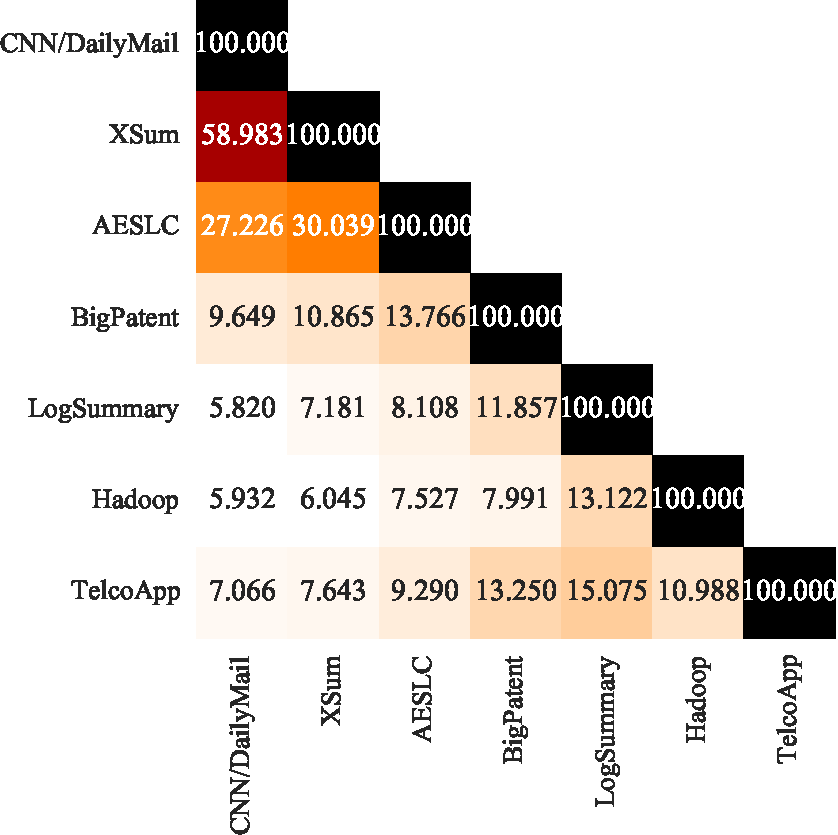
\includegraphics[width=.75\textwidth]{images/thesis/500_vocab_overlap_correlation}
\caption{Top 500 most frequent tokens (excluding stop words and infrequent tokens) shared among datasets from different domains.}
\label{fig:datasets_vocab_overlap}
\end{figure}

CNN/DailyMail and XSum share the highest amount of frequent tokens,
which is not unexpected as they are both datasets for news summarization.
AESLC shares a considerable amount of frequent tokens with those domains,
but otherwise the overlap between datasets is quite limited.

In general, the vocabulary of log datasets differs from that of other domains.
Log datasets show highest similarities between themselves,
but are quite diverse even among themselves.
A model performing well on one of these datasets might therefore not perform well on the other log datasets.
Interestingly, the vocabulary of BigPatent shows moderate similarity with \telco{} and \logsummary{},
which we find promising in respect to the transferability of log summarization.

\section{Investigating the Effects of Separators on Output Quality}\label{sec:preliminary_separators}

In \autoref{subsec:preprocessing} on \autopageref{subsubsec:model_input_challenges} we highlighted some challenges that come with
separating log messages from one another in the models' input;
Log messages often do not form complete sentences and thus punctuation cannot reliably be used for the purpose of separating messages.

Without such a separator it will be impossible for us to tell
where a model intends to end a log message and begin the next one,
as well as it being difficult for models to distinguish the semantic content of individual log messages.

In this section, we aim to find a sequence of tokens that can adequately serve as
separators for each model.

\subsection{Experimental setup}

Ideally, the separators we consider also have the function of separating text sequences
with different semantic content in the natural language corpora the models have been trained on.
We hypothesize that a model is more likely to understand that the additional tokens
are used to syntactically separate log messages which are text segments of different semantic contents.

We consider the following options:
\begin{description}
\item[\acs{bos}-/\acs{eos} tokens] These tokens are used to signify the beginning and end of the model's input.
      When fine-tuned for certain sentence-pair classification tasks \citeauthor*{bart} use their \ac{eos}-token as separator~\parencite[7874]{bart}.
      PEGASUS has a designated \ac{eos}-token only.

      This approach is equivalent to passing each log messages separately to a model's tokenizer and then manually concatenating the results.
\item[semicolons] Semicolons may be used in written text; usually they are used to separate two related but independent text segments.%
      \footnote{See \accessurl{https://www.grammarly.com/blog/semicolon/}{13.04.2022} for exemplified uses in the English language.}
      A semicolon used this way is typically separated by a space from the next word.
      BART's tokenizer makes the distinction between a semicolon with a subsequent space or without, while PEGASUS' does not.
\item[newlines] PEGASUS is able to encode newlines in its input,
      which separate paragraphs in the pre-training data.
      The special newline-token also has the benefit of not being contained in any log messages,
      as newlines typically separate different log-entries.
      Thus we can guarantee that newlines are only used to separate different log messages,
      while the model should still be familiar with the semantic meaning of a newline.
\end{description}
For better comparison we also include a space as a baseline to compare
model performances for when no special separator is employed.

We use \bart{-Large} and \pegasus{-Large} for this preliminary experiment,
which have not been fine-tuned to any specific task,
and train the models with the same setup as later in the \acs*{fsl} setting later described in \autoref{sec:evaluation_experiment_finetuned},
apart from the separator used to join log messages in the model inputs and reference summaries.
To be able to anticipate the effects of different separators on performance directly,
we decide to evaluate the models' text generation capabilities and against investigating perplexity.
Hence we perform a rough hyperparameter search to find \enquote{good-enough} parameters for the beam-search used to generate text.

\subsection{Results}

As the metric scores from this experiment are not meant to be comparable with the results from other experiments in this work,
but rather to evaluate different separators for each model individually,
we feel free to report the models' performance on a smaller, manually chosen validation set for each dataset.
(36, 25 and 11 examples for \logsummary{}, \hadoop{} and \telco{} respectively.)
Additionally we only report mean \(F_1\)-scores for \acs*{rouge}-1, \acs*{rouge}-2 and sentence-level \acs*{rouge}-L
since we are primarily focused on observing any relative improvements,
not conducting a comprehensive evaluation of the models.

We chose sentence-level \acs*{rouge}-L rather than summary-level,
as we are interested in the models ability to present the information in the same order as in the reference,
which would be ignored by summary-level \acs*{rouge}-L.

The results for BART are reported in \autoref{tab:separators_bart},
while the results for PEGASUS are shown in \autoref{tab:separators_pegasus}.
The best results are highlighted.

\begin{table}[htbp]
\centering
\footnotesize
\begin{tabular}{lccc}
                                 & \multicolumn{3}{c}{\scriptsize{}\acs*{rouge}-1 / \acs*{rouge}-2 / \acs*{rouge}-LSent}\\
                                 & \h{\logsummary{}}          & \h{\hadoop{}}              & \h{\telco{}}\\
\midrule
space (no syntactic separation)  & 71.6/63.2/68.2             & 35.5/31.6/34.1             & \h{43.8}/\h{37.1}/\h{38.7}\\
\acs{bos}-/\acs{eos}-token pair  & 55.9/45.0/53.3             & 33.7/28.0/31.0             & 35.1/27.5/27.6\\
% \acs{bos}-token                  & 51.2/33.3/50.2             & 42.0/34.8/39.5             & 38.4/31.0/33.8\\
semicolon with space             & 67.2/58.1/59.4             & 36.5/30.1/34.8             & 37.2/29.2/29.8\\
semicolon without space          & \h{72.4}/\h{65.7}/\h{70.4} & \h{47.6}/\h{40.2}/\h{45.2} & \h{43.8}/36.1/38.1\\
% double space                     & \h{77.5}/\h{68.4}/\h{71.6} & 37.5/31.1/35.2             & 30.7/23.5/26.5\\
\end{tabular}
\caption{Mean \acs*{rouge}-scores using \bart{-Large} with different separators across all validation sets.}
\label{tab:separators_bart}
\end{table}

\begin{table}[htbp]
\centering
\footnotesize
\begin{tabular}{lccc}
                                 & \multicolumn{3}{c}{\scriptsize{}\acs*{rouge}-1 / \acs*{rouge}-2 / \acs*{rouge}-LSent}\\
                                 & \h{\logsummary{}}          & \h{\hadoop{}}              & \h{\telco{}}\\
\midrule
space (no syntactic separation)  & 69.4/60.7/65.4             & 31.6/28.7/31.5             & 26.5/20.4/24.2\\
\acs{eos}-token                  & 51.8/42.3/51.8             & 21.9/18.9/21.8             & \phantom{0}7.6/\phantom{0}5.4/\phantom{0}7.1\\
semicolon                        & \h{77.0}/68.1/\h{72.7}     & \h{33.0}/\h{30.0}/\h{32.7} & 23.8/19.2/23.0\\
newline                          & 76.9/\h{68.8}/71.8         & 23.6/20.2/23.4             & \h{29.1}/\h{25.1}/\h{28.6}\\
\end{tabular}
\caption{Mean \acs*{rouge}-scores using \pegasus{-Large} with different separators across all validation sets.}
\label{tab:separators_pegasus}
\end{table}

We also report the ratio of log messages ending in a punctuation mark (one of \verb+.?!+) in \autoref{tab:sentence_endings},
and the ratio of log messages starting with a capital letter in \autoref{tab:capital_beginnings}.

\begin{table}[htbp]
\centering
\footnotesize
\begin{tabular}{ccc}
\h{\logsummary{}}                     & \h{\hadoop{}}                         & \h{\telco{}}\\
\midrule
\(\frac{311}{12020} \approx 2.587\%\) & \(\frac{233}{25931} \approx 0.899\%\) & \(\frac{592}{6079} \approx 9.738\%\)
\end{tabular}
\caption{Ratio of log messages ending in a punctuation mark across all datasets.}
\label{tab:sentence_endings}
\end{table}

\begin{table}[htbp]
\centering
\footnotesize
\begin{tabular}{ccc}
\h{\logsummary{}}                       & \h{\hadoop{}}                            & \h{\telco{}}\\
\midrule
\(\frac{5479}{12020} \approx 45.582\%\) & \(\frac{23550}{25931} \approx 90.818\%\) & \(\frac{1970}{6079} \approx 32.407\%\)
\end{tabular}
\caption{Ratio of log messages starting with a capitalized token across all datasets.}
\label{tab:capital_beginnings}
\end{table}

\subsection{Discussion}

Generally, \acs{bos}-/\acs{eos}-tokens perform poorly as separators,
in all cases performing worse than providing no syntactical separation of log messages.
The poor performance can at least in part be explained by the fact
that \acs{eos}-tokens signify to the beam-search that a beam is finished.
When manually inspecting the generated summaries, we notice they are particularly short,
leading to low recall, resulting in a low overall score.

In most cases, providing some form of separators significantly improved performance compared to using no explicit syntactical separation,
confirming our assumption that it is important for models to be able to differentiate between different log messages.
In settings where spaces performed comparatively well,
we suspect that models may be able to use existing patterns concerning punctuation or capitalization to distinct between log messages.

\paragraph{PEGASUS}

We observe that \pegasus{-Large} clearly benefits from the use of explicitly inserted separators on every dataset.
This can be seen well on the \logsummary{}-dataset,
where either option resulted in a minimum of a \(9.79\%\) increase in model performance after training (among all observed metrics)
compared to separating subsequent log messages by a space.

Interestingly, not providing additional syntactical separation by using spaces as separators
performs well with \hadoop{}.
We believe this can in part be explained by the consistent use of capitalization in this dataset,
as signified by the high rate of capital letters at the beginning of log messages.
Our hypothesis is that \pegasus{-Large} picked up on this pattern and it is sufficient for it to identify semantically different text segments.

On the other hand, the low amount of punctuation at the end of log messages seen in \hadoop{}
may be the reason why using a punctuation-symbol such as semicolons performs better than using newlines in this specific case,
whereas introducing extra punctuation performs worse in cases where punctuation is already present,
such as \telco{}.

\paragraph{BART}

With \bart{-Large}, the benefits of introducing explicit separators seem less pronounced
considering that spaces almost as well as the best choice for \logsummary{} and the best for \telco{}.

However, we do also see a minimum of \(27.22\%\) performance increase for all considered metrics on the \hadoop{}-dataset
when using semicolons without additional spaces compared to using spaces for separation.\\
This shows to us that \bart{-Large} also benefits from being able to differentiate between independent log messages,
at least in cases where there is a lack of punctuation at the end of messages.

Oddly enough, inserting a semicolon followed by a space between each log message,
as one would do to separate independent text segments in a sentence, performs poorly.
We are unsure why the model prefers semicolons without subsequent spaces,
although we will highlight that the semicolon is represented by different tokens with different embeddings
depending on whether a space is inserted or not.
This means that the model did not necessarily learn that these two tokens have the same meaning for humans,
instead there may be some biases present in the pre-training data that make the semicolon without a space
a better syntactic separator of semantically independent text segments.

\paragraph{Conclusion}

It is impracticable to evaluate all possible tokens as separators.
Hence, there may be some other sensible choices
we did not consider that are better suited for use as separators.
Furthermore, models previously fine-tuned may prefer different separators depending on the patterns seen in their domain and dataset.
Nevertheless, performing such a preliminary study for each fine-tuned summarization model from \autoref{tab:finetuned_models_overview}
individually would be an impractical effort;
instead we rely on the assumption that previously fine-tuned models inherit some knowledge on separators from their pre-trained bases.

Our goal was not to find optimal separators for our models,
but to find ones that produce adequate results.
Ideally, we would like to choose a single option per model going forward and use it consistently across all datasets.
It would allow for models to be used in more universal settings.

We make an exception for this rule with PEGASUS-models:
We choose newlines as separators for \logsummary{} and \telco{}-datasets,
but use semicolons on the \hadoop{}-dataset
because we see a significant \(39.74\%\) increase among all observed metrics compared to newlines.

For BART-models we decide on semicolons as separators (without inserting a space after each semicolon)
for all datasets, even if slightly outperformed by using regular spaces on \telco{}.

As not introducing additional syntactic separation makes it harder to tell apart independent text segments in the summary
and therefore decreases readability,
we believe using spaces as separators is less helpful for any human operators using the model as it,
even if the performance is comparatively good when considering \acs*{rouge} metrics.

\section{Evaluation of Summarization Models from other Domains}\label{sec:evaluation_experiment_finetuned}

As motivated in \autoref{subsubsec:approch_experiment_1},
we aim to determine if models fine-tuned for summarization on other previously researched domains
are able to transfer their knowledge on summarization to log-data.

For this, we evaluate all models laid out in \autoref{tab:finetuned_models_overview}
on \autopageref{tab:finetuned_models_overview}
in a \ac{zsl} and a \ac{fsl} setting.
Additionally, we include the baseline models \bart{-Large} and \pegasus{-Large}
which have not been fine-tuned on summarization before.
This way, we can see if previous fine-tuning for summarization makes a noticeable difference in performance,
or if it suffices to fine-tune on the limited data available.

Under ideal circumstances we could simply let each of the models generate summaries on all our datasets.
Using the \acs*{rouge}-metrics we could then quantify the performance of the models
and conclude if any singular model outperforms the others.

During preliminary experiments, however, we find that the length of generated text heavily
depends on the parameter chosen for the beam-search,
such as constraints on the minimum and maximum amount of tokens generated
and the \emph{length penalty} in particular.
The length of the summary directly influences its quality according to the \acs*{rouge}-metrics;
As such we would need to find optimal values for such parameters influencing the generation of text
in order to keep a fair comparison between models.
Unfortunately, each model variant appears to have their own optima for such generation-parameters on every dataset.

Because finding optimal values for these parameters for each model is error-prone and cumbersome,
we instead choose to initially focus on the perplexity for comparing different models,
then compare generated summaries for selected models only.

Sometimes we employ boxplots to visualize our results;
these are the classic \enquote{Tukey} boxplots~\parencite{boxplots},
with a red line indicating the median of the distribution.
Similarly, we use violin plots that visualize the data's distribution density,
using the same indication of the median.
Both types of plots and their origins are explained in \parencite{boxplots}.

We include intermediate results and frequently draw similar conclusions from different perspectives.
We believe this to be necessary to justify the decisions we take in presenting the final results,
but as a consequence, this section may be a bit long-winded.\\
As such we summarize any important intermediate conclusions during the final discussion of this experiment in
\autoref{subsec:evaluation_experiment_finetuned_discussion}.

\subsection{Experimental Setup}

During the experiments in the next segments,
we regularly evaluate models in two different settings with differing levels of supervision;
With further fine-tuning on the training dataset or without:

\paragraph{\acf*{zsl} setting}

As described in \autoref{subsec:training_test_split}
we defined a set of training examples for each dataset and use the rest for evaluation.

A \acl{zsl} setting means that the models have previously seen zero training examples on the concrete task/dataset used;
as such we simply run the models on the test datasets and evaluate their outputs,
either through perplexity or through examining their summaries generated via beam-search.

Following \citeauthor*{bart} and \citeauthor*{pegasus} we apply a label smoothing factor of \(0.1\)
for computing the cross-entropy loss~\parencites[7876]{bart}[appendix]{pegasus},
which impacts the perplexity scores.

\paragraph{\acf*{fsl} setting}

In the \ac{fsl} setting we first train the models on a small training set,
minimizing the cross-entropy between model predictions and reference summaries,
and then evaluate it on the same test set as described above.

We use an effective batch-size of 8 and using a constant learning rate of \(5 \cdot 10^{-5}\) we train for different amount of steps on each dataset:
\begin{description}[nosep, itemsep=1ex, labelwidth=\widthof{\logsummary}, leftmargin=\labelwidth+\labelsep, align=parright]
\item[\logsummary] \(20 \cdot \left\lceil\frac{30}{8}\right\rceil = 80\)
\item[\hadoop]     \(15 \cdot \left\lceil\frac{50}{8}\right\rceil = 105\)
\item[\telco]      \(25 \cdot \left\lceil\frac{16}{8}\right\rceil = 50\)
\end{description}
where the number of steps is determined as
\begin{equation}
\text{\#steps} = \text{\#epochs} \cdot \left\lceil\frac{\text{\#training-examples}}{\text{batch-size}}\right\rceil
\end{equation}
An epoch is understood as an iteration over the entire training dataset.
We chose an adequate number of epochs using our experiences from preliminary trials,
where we observed roughly at which point the generation
performance starts to stagnate or even deteriorate on a validation set
and chose an amount of epochs that works for \emph{both} model architectures.

\subsection{Analysis of Model Perplexities}

We first evaluate the perplexity of the models only.
Again, perplexities are not comparable between models with different vocabularies
for the reasons laid out in \autoref{sec:perplexity}.
However, we can compare models of the same architecture,
e.g. \bart{-Large} with \bart{-CNN} as they use the same vocabulary and tokenizer.

The results for BART are shown in \autoref{tab:bart_zsl_perplexities} for the \acl{zsl} setting
and in \autoref{tab:bart_fsl_perplexities} for the \acl{fsl} setting.

\begin{table}[htbp]
\centering
\footnotesize
\begin{tabular}{lrrr}
              & \h{\logsummary{}} & \h{\hadoop{}} & \h{\telco{}}\\
\midrule
\bart{-Large} & 869.696           & 19.356        & 31.837\\
\bart{-CNN}   & \h{89.208}        & \h{5.447}     & \h{7.373}\\
\bart{-XSum}  & 412.338           & 10.316        & 11.844\\
\end{tabular}
\caption{Perplexities of BART variants in a  \acl*{zsl} setting.}
\label{tab:bart_zsl_perplexities}
\end{table}

\begin{table}[htbp]
\centering
\footnotesize
\begin{tabular}{lrrr}
              & \h{\logsummary{}} & \h{\hadoop{}} & \h{\telco{}}\\
\midrule
\bart{-Large} & \h{15.547}    & 4.581         & 7.151\\
\bart{-CNN}   & 17.236        & \h{4.369}     & \h{6.009}\\
\bart{-XSum}  & 15.820        & 4.518         & 7.032\\
\end{tabular}
\caption{Perplexities of BART variants in a  \acl*{fsl} setting.}
\label{tab:bart_fsl_perplexities}
\end{table}

For PEGASUS we report the \acl{zsl} results in \autoref{tab:pegasus_zsl_perplexities}
and in \autoref{tab:pegasus_fsl_perplexities} for the \acl{fsl} setting.

\begin{table}[htbp]
\centering
\footnotesize
\begin{tabular}{lrrr}
                     & \h{\logsummary{}} & \h{\hadoop{}} & \h{\telco{}}\\
\midrule
\pegasus{-Large}     & 1684.929      & \h{100.972}   & \h{168.063}\\
\pegasus{-CNN}       & 563.526       & 136.606       & 173.432\\
\pegasus{-XSum}      & \h{495.076}   & 525.619       & 459.367\\
\pegasus{-AESLC}     & 747.233       & 703.096       & 744.069\\
\pegasus{-BigPatent} & 1399.012      & 705.201       & 330.518\\
\end{tabular}
\caption{Perplexities of PEGASUS variants in a  \acl*{zsl} setting.}
\label{tab:pegasus_zsl_perplexities}
\end{table}

\begin{table}[htbp]
\centering
\footnotesize
\begin{tabular}{lrrr}
                     & \h{\logsummary{}} & \h{\hadoop{}} & \h{\telco{}}\\
\midrule
\pegasus{-Large}     & 12.957        & 6.115         & 32.345\\
\pegasus{-CNN}       & \h{12.244}    & \h{5.559}     & \h{27.920}\\
\pegasus{-XSum}      & 13.144        & 9.560         & 78.193\\
\pegasus{-AESLC}     & 19.775        & 8.943         & 68.682\\
\pegasus{-BigPatent} & 60.724        & 29.735        & 108.614\\
\end{tabular}
\caption{Perplexities of PEGASUS variants in a  \acl*{fsl} setting.}
\label{tab:pegasus_fsl_perplexities}
\end{table}

Generally, we notice that previous fine-tuning on summarization data does help when in a \ac{zsl} setting,
but the differences between models shrink significantly after training on the few examples provided.

This is especially true for BART models,
for which the largest relative deviation between the best and lowest scoring models after fine-tuning is
approximately \(11\%\) on the \logsummary{}, \(5\%\) on the \hadoop{} and \(19\%\) on the \telco{}-dataset.
(Which is low compared to for example \(\approx 255\%\) on the \hadoop{} dataset for \ac{zsl}.)
While judging the perplexity alone is not enough to infer a models performance to generate good summaries,
this is a strong indicator that previous training for summarization
does not contribute considerably to a models ability to predict summaries on our specific log-data.

This also holds for PEGASUS, where \pegasus{-Large} always shows the second-best performance,
with an approximate relative derivation of \(6\%\), \(10\%\) and \(16\%\)
from \pegasus{-CNN} on \logsummary{}, \hadoop{} and \telco{} respectively.

However, we can see that using previously fine-tuned models
can actually perform substantially worse than the baseline \pegasus{-Large}.
Especially the variant fine-tuned for summarization on BigPatent failed to achieve similar perplexities as the other variants,
despite the higher overlap of vocabulary we found in \autoref{subsec:other_domains_vs_log_datasets}.
As summaries in BigPatent tend to be abstractive~\parencite[2204-2205]{bigpatent},
we suspect that the model is unable to quickly adapt to a more extractive task such as the ones presented by us.
\pegasus{-BigPatent} may improve further with more fine-tuning steps,
but even so, \pegasus{-Large} managed to adapt much quicker:
Initially staring with a higher perplexity in the \ac{zsl} setting,
but achieving a significantly better \ac{fsl} result after the same amount of training-steps on \logsummary{}.
This reinforces our assessment that further fine-tuning models previously trained on summarization tasks
is not worth it for dissimilar domains such as log-data
and that fine-tuning pre-trained models even with only a few examples is sufficient.

Still, for both models the best performing \ac{fsl} model
is most often the variant trained on the CNN/DailyMail dataset,
albeit closely followed by the baselines \bart{-Large} and \pegasus{-Large}.

Extractive models tend to perform better on the CNN/DailyMail news-dataset than abstractive ones~\parencite[547]{summarization_critical_evaluation},
which may explain why models fine-tuned on this dataset outperform those trained on other domains.
After all, the summaries in all our log summarization datasets are purely extractive,
hence do not include any novel words not seen in the input data or any paraphrasation of content.
The slight difference in performance compared to the baselines not tuned for summarization
might indicate that there is still some insight to gain concerning which text segments are relevant.
We believe this is why we are seeing that \bart{-CNN} performs comparatively well in a \ac{zsl} setting.

As noted before, lower perplexity usually correlates with better performance in applications,
but if the model simply gets more confident in more obvious cases, this is not always the case.
Hence we cannot be sure that the models showing the best perplexities
are also the ones performing the best for summarization of our log-data.
To select the best models, we conduct a few further trials before decide on the final models to evaluate.

\subsection{Further Trials to determine the best Models}

\paragraph{PEGASUS}
Due to the summary length heavily impacting the recall of the \acs*{rouge} metric,
and the complications arising from optimizing the summary length using the parameters of the beam-search,
we instead decide to compare only the \acs*{rouge} precision
while setting the length of generated summaries to a small, fixed amount.
For the PEGASUS models we decide on the following lengths:
\begin{itemize}
\item We let the models generate exactly 20 tokens on the \telco{} and \hadoop{} datasets.
\item On the \logsummary{} dataset, we instruct the model to generate only 8 tokens,
      as summaries are much shorter in this dataset.
      8 tokens corresponds to the median length of summaries using PEGASUS' tokenizer.
\end{itemize}

By comparing the precision only, we can judge what percentage of the few written tokens are actually relevant.
Thus we hope to anticipate the performance of the models when scaled up to the full summarization task
and select a well-performing model.

The mean \(F_1\)-scores for \acs*{rouge}-1, \acs*{rouge}-2 and sentence-level \acs*{rouge}-L
are reported in \autoref{tab:pegasus_trial_zsl} for the \ac{zsl} setting
and in \autoref{tab:pegasus_trial_fsl} for the \ac{fsl} one.

\begin{table}[htbp]
\centering
\footnotesize
\begin{tabular}{lccc}
                     & \multicolumn{3}{c}{\scriptsize{}\acs*{rouge}-1 / \acs*{rouge}-2 / \acs*{rouge}-LSent}\\
                     & \h{\logsummary{}}          & \h{\hadoop{}}              & \h{\telco{}}\\
\midrule
\pegasus{-Large}     & 50.9/27.2/48.2             & 75.3/\h{72.6}/75.1         & \h{43.3}/\h{34.2}/\h{42.9}\\
\pegasus{-CNN}       & \h{58.9}/\h{32.9}/\h{55.1} & \h{77.8}/70.8/\h{77.7}     & 39.5/27.2/37.9\\
\pegasus{-XSum}      & 41.0/25.5/39.3             & 66.0/60.9/65.6             & 26.9/12.0/24.9\\
\pegasus{-AESLC}     & 41.8/23.7/39.5             & 46.1/33.4/45.9             & 31.0/15.4/29.3\\
\pegasus{-BigPatent} & 15.7/\phantom{0}8.5/14.9   & 25.3/\phantom{0}5.0/25.1   & 14.3/\phantom{0}2.0/11.7\\
\end{tabular}
\caption{Mean \acs*{rouge} precisions of \ac*{zsl} PEGASUS models in a constrained summarization task.}
\label{tab:pegasus_trial_zsl}
\end{table}

\begin{table}[htbp]
\centering
\footnotesize
\begin{tabular}{lccc}
                     & \multicolumn{3}{c}{\scriptsize{}\acs*{rouge}-1 / \acs*{rouge}-2 / \acs*{rouge}-LSent}\\
                     & \h{\logsummary{}}          & \h{\hadoop{}}              & \h{\telco{}}\\
\midrule
\pegasus{-Large}     & \h{82.5}/\h{70.7}/\h{78.3} & \h{94.2}/\h{93.4}/\h{94.1} & \h{49.4}/\h{38.6}/\h{48.5}\\
\pegasus{-CNN}       & 81.0/69.6/77.9             & 93.5/82.7/89.6             & 44.3/32.3/43.1\\
\pegasus{-XSum}      & 81.7/69.4/77.6             & 92.9/89.7/92.7             & 45.4/30.0/43.2\\
\pegasus{-AESLC}     & 79.0/64.6/75.3             & 92.5/91.1/92.4             & 47.7/31.1/45.9\\
\pegasus{-BigPatent} & 49.8/34.1/48.5             & 46.4/29.7/44.7             & 32.9/19.5/29.9\\
\end{tabular}
\caption{Mean \acs*{rouge} precisions of \ac*{fsl} PEGASUS models in a constrained summarization task.}
\label{tab:pegasus_trial_fsl}
\end{table}

We observe that the perplexity of a model does not perfectly match its performance in this constrained summarization setting:
In the \ac{zsl} setting, \pegasus{-Large} performs second-best on \telco{} despite previously showing the highest perplexity.
On the other side of the spectrum, \pegasus{-BigPatent} performs worse than its perplexity would indicate;
for example in the \telco{}-dataset where the \ac{fsl} BigPatent model performs about as good
as the AESLC model in the \ac{zsl} setting,
despite \pegasus{-BigPatent} now exhibiting a perplexity that is about 7 times lower than \ac{zsl} \pegasus{-AESLC}.

Unsurprisingly, the models perform much better in a \ac{fsl} setting after being fine-tuned on a few examples.
We explore the quality of these generated texts in an example from the \logsummary{}-dataset in \autoref{tab:logsummary_pegasus_example_1}.

\begin{table}[htbp]
\centering
\footnotesize
\setlength{\tabcolsep}{.5ex}
\begin{tabularx}{\textwidth}{XXXXX}
\toprule
\multicolumn{4}{c}{\textbf{input}}
&\textbf{reference summary}\\
\midrule
\multicolumn{4}{p{.75\textwidth}}{
\tiny
\ttfamily\hbadness=10000
Accepted socket connection from remote host \#83617

Connection request from old client remote host \#83617 ; will be dropped if server is in r-o mode

Client attempting to establish new session at remote host \#83617

Established session 238367163526545476 with negotiated timeout 10000 for client remote host \#83617

\textelp{} \textit{(messages repeat with 4 different clients)}}
&
\tiny
\ttfamily\hbadness=10000
Accepted socket connection

Connection request

Established session timeout
\\
\midrule
\h{\pegasus{-Large}}
&\h{\pegasus{-CNN}}
&\h{\pegasus{-XSum}}
&\h{\pegasus{-AESLC}}
&\h{\pegasus{-BigPat.}}\\
\tiny\acs*{rouge}-LSent precision: \(100\)
&\tiny\acs*{rouge}-LSent precision: \(60\)
&\tiny\acs*{rouge}-LSent precision: \(16.7\)
&\tiny\acs*{rouge}-LSent precision: \(40\)
&\tiny\acs*{rouge}-LSent precision: \(33.3\)\\
\midrule
\tiny
\ttfamily\hbadness=10000
Accepted socket connection

Established session
&
\tiny
\ttfamily\hbadness=10000
Accepted socket connection

Client attempting
&
\tiny
\ttfamily\hbadness=10000
Client attempting to establish new session
&
\tiny
\ttfamily\hbadness=10000
Connection request from old client
&
\tiny
\ttfamily\hbadness=10000
A socket request from old client\\
\bottomrule
\end{tabularx}
\caption{\ac*{fsl} predictions on an example from the \emph{ZooKeeper}-subdataset of \logsummary{}.}
\label{tab:logsummary_pegasus_example_1}
\end{table}

We find that, at least with this example,
models originating from a more abstractive summarization background prefer to include grammatically sound segments in their summary,
as can be seen for \pegasus{-XSum} and \pegasus{-BigPatent}.

\pegasus{-BigPatent}'s summary is the most abstractive one, combining two different log messages into a single statement.
This hurts its score on the \acs{rouge} metric, even if the summary is analogous to the one from \pegasus{-AESLC},
and explains why this model performs poorly regarding this metric.

However, this more abstractive approach is also more error-prone.
In another example, \autoref{tab:logsummary_pegasus_example_2}, \pegasus{-BigPatent} includes additional descriptive text,
which does not fit the context of the log:
\verb+binding to port+ is an action taken by the software producing the log,
but similar to the summaries of patents in the BigPatent dataset,
the model seems to interpret the log as a procedure that needs to be described.

Therefore we do not believe that abstractive models perform worse solely because the \acs*{rouge} metric prefers extractive summaries,
but because they do not fully understand the log-data presented to them and fail to interpret it in a meaningful way;
even more so as they have not been provided with abstractive summaries during fine-tuning.
Ultimately we think a purely extractive summary in the style of the human-written summaries of this dataset will be more helpful to any human operator
than a factually inconsistent abstractive description of what happened.

Hence why we decide to select the \pegasus{-Large} model for further evaluation:
Comparing \autoref{tab:pegasus_trial_fsl} and \autoref{tab:pegasus_trial_zsl}, it outperforms every other variant in the \ac{fsl} setting and is competitive in the \ac{zsl} setting.
As can be seen from the examples, its summaries follow the extractive style of the human-written summaries.

\pegasus{-CNN} would be another viable alternative, as it shows even better perplexity,
but evidently it performs slightly worse in this constrained generation setting.
We speculate this is the case because \pegasus{-Large} can more quickly adapt to the summarization task,
as it does not have any prior biases towards which parts of the input document need to be included in the summary.
Previous research has shown that summarization of news articles is prone to substantial layout biases~\parencite[544]{summarization_critical_evaluation},
speaking against the use of previously fine-tuned models such as \pegasus{-CNN},
which is accustomed to summarizing news articles.

\begin{table}[htbp]
\centering
\footnotesize
\setlength{\tabcolsep}{.5ex}
\begin{tabularx}{\textwidth}{XXXXX}
\toprule
\multicolumn{4}{c}{\textbf{input}}
&\textbf{reference summary}\\
\midrule
\multicolumn{4}{p{.75\textwidth}}{
\tiny
\ttfamily\hbadness=10000
binding to port remote host \#44607remote host \#5137

tickTime set to 2000

minSessionTimeout set to -1

maxSessionTimeout set to -1

initLimit set to 10

Reading snapshot zookeeper

My election bind port : remote host \#44607remote host \#47103

LOOKING

New election. My id = 1 , proposed zxid = 30064771479

Notification : 1 ( n.leader ) , 30064771479 ( n.zxid ) , 1 ( n.round ) , LOOKING ( n.state ) , 1 ( n.sid ) , 7 ( n.peerEPoch ) , LOOKING ( my state )

Have smaller server identifier , so dropping the connection : ( 2 , 1 )

Received connection request remote host \#46154

Have smaller server identifier , so dropping the connection : ( 3 , 1 )

Received connection request remote host \#7574

Notification : 3 ( n.leader ) , 30064771479 ( n.zxid ) , 1 ( n.round ) , LOOKING ( n.state ) , 2 ( n.sid ) , 7 ( n.peerEPoch ) , LOOKING ( my state )

\textelp{} \textit{(4 similar messages discarded in this example for brevity)}

Notification : 3 ( n.leader ) , 30064771479 ( n.zxid ) , 1 ( n.round ) , FOLLOWING ( n.state ) , 2 ( n.sid ) , 7 ( n.peerEPoch ) , LOOKING ( my state )
}
&
\tiny
\ttfamily\hbadness=10000
binding to port

Reading snapshot

Have smaller server identifier

dropping the connection

Received connection request
\\
\midrule
\h{\pegasus{-Large}}
&\h{\pegasus{-CNN}}
&\h{\pegasus{-XSum}}
&\h{\pegasus{-AESLC}}
&\h{\pegasus{-BigPat.}}\\
\tiny\acs*{rouge}-LSent precision: \(100\)
&\tiny\acs*{rouge}-LSent precision: \(40\)
&\tiny\acs*{rouge}-LSent precision: \(60\)
&\tiny\acs*{rouge}-LSent precision: \(100\)
&\tiny\acs*{rouge}-LSent precision: \(50\)\\
\midrule
\tiny
\ttfamily\hbadness=10000
Have smaller server identifier

Received
&
\tiny
\ttfamily\hbadness=10000
bind to port remote host
&
\tiny
\ttfamily\hbadness=10000
My state

Received connection request
&
\tiny
\ttfamily\hbadness=10000
binding to port

Received connection
&
\tiny
\ttfamily\hbadness=10000
A method for binding to port\\
\bottomrule
\end{tabularx}
\caption{\ac*{fsl} predictions on a more diverse example from the \emph{ZooKeeper}-subdataset of \logsummary{}.}
\label{tab:logsummary_pegasus_example_2}
\end{table}

\paragraph{BART}
For the BART variants, the performances on this constrained generation task do not differ significantly between models,
so we chose to omit the results here.
Instead, we did perform a hyperparameter search for all variants on the \logsummary{} task,
where the generated summaries are the shortest,
and thus the search can evaluate different parameters in a relatively timely manner.
To further speed up the search,
it is performed on a manually selected validation set and not the whole dataset,
resulting in 20 trials to determine an optimal length penalty.
The resulting \acs*{rouge}-2 and summary-level \acs*{rouge}-L metrics on the evaluation dataset are visualized
in \autoref{fig:bart_trial_zsl_logsummary} (\acs{zsl}) and \autoref{fig:bart_trial_fsl_logsummary} (\acs{fsl}).

\begin{figure}[htbp]
\centering
\subfloat[\bart{-Large}]{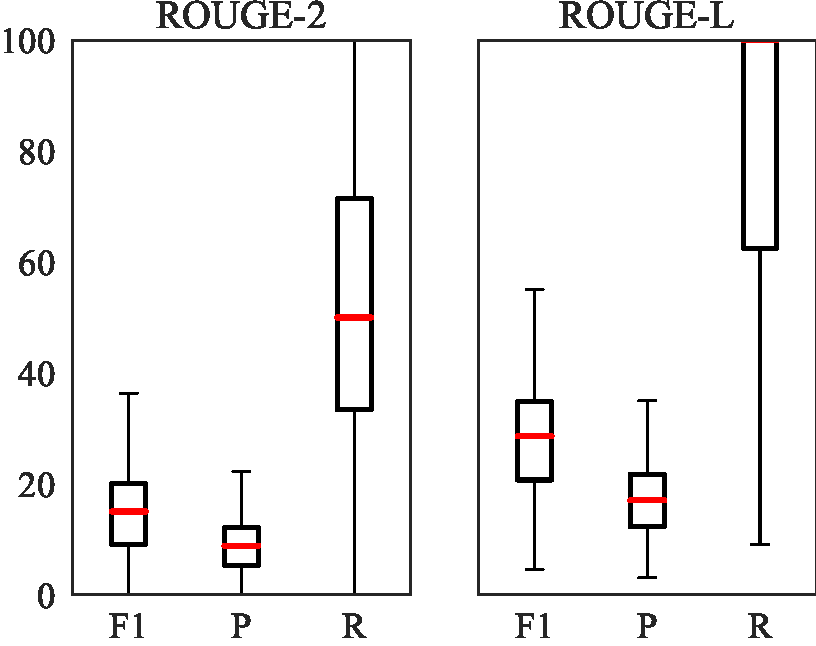
\includegraphics[width=.32\textwidth]{images/thesis/result_boxplots/logsummary_bart-large-zsl}}%
\hfill{}%
\subfloat[\bart{-CNN}]{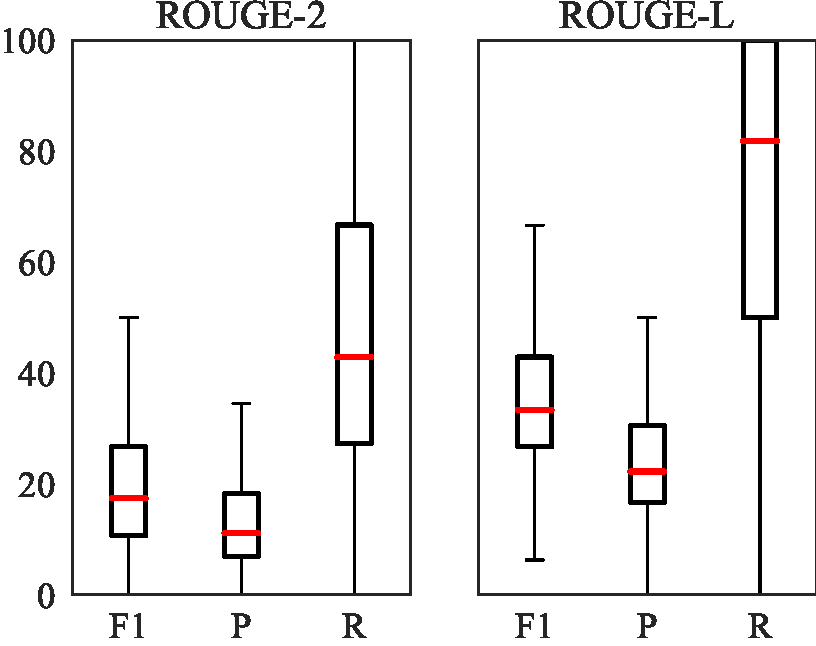
\includegraphics[width=.32\textwidth]{images/thesis/result_boxplots/logsummary_bart-large-cnn-zsl}}%
\hfill{}%
\subfloat[\bart{-XSum}]{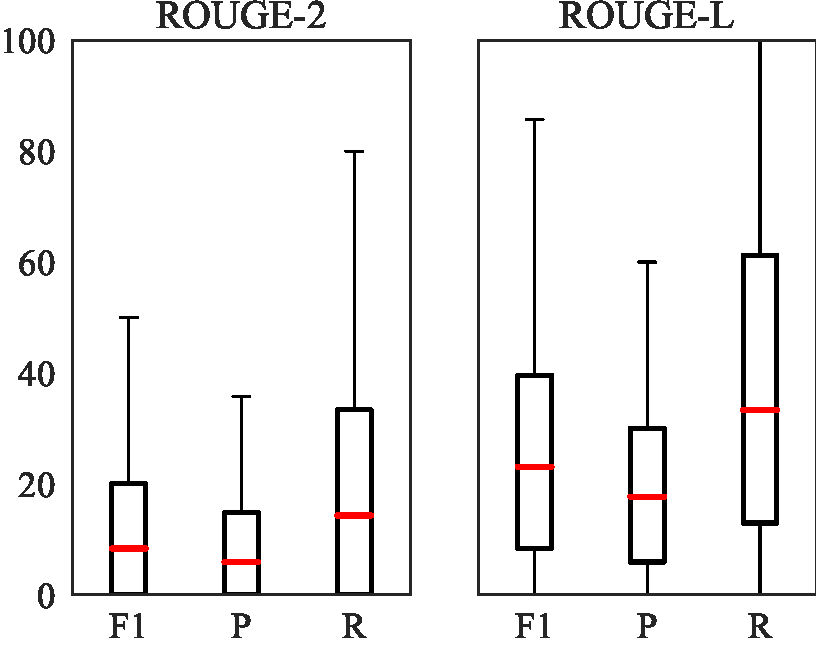
\includegraphics[width=.32\textwidth]{images/thesis/result_boxplots/logsummary_bart-large-xsum-zsl}}
\caption{Boxplots showing \acs*{rouge} recall, precision and \(F_1\)-scores
for different BART variants without further fine-tuning (\acs*{zsl}) on the \logsummary{} dataset.}
\label{fig:bart_trial_zsl_logsummary}
\end{figure}

\begin{figure}[htbp]
\centering
\subfloat[\bart{-Large}]{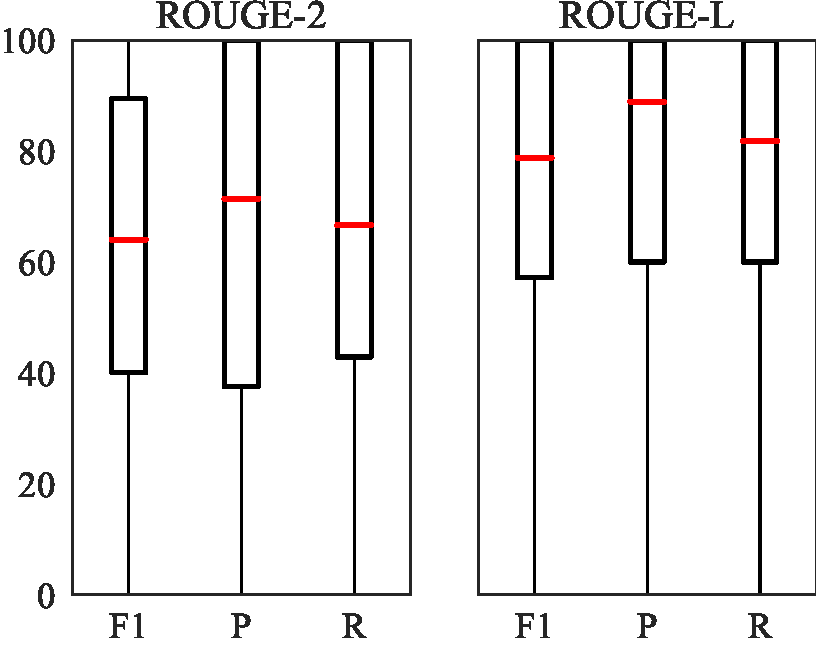
\includegraphics[width=.32\textwidth]{images/thesis/result_boxplots/logsummary_bart-large}}%
\hfill{}%
\subfloat[\bart{-CNN}]{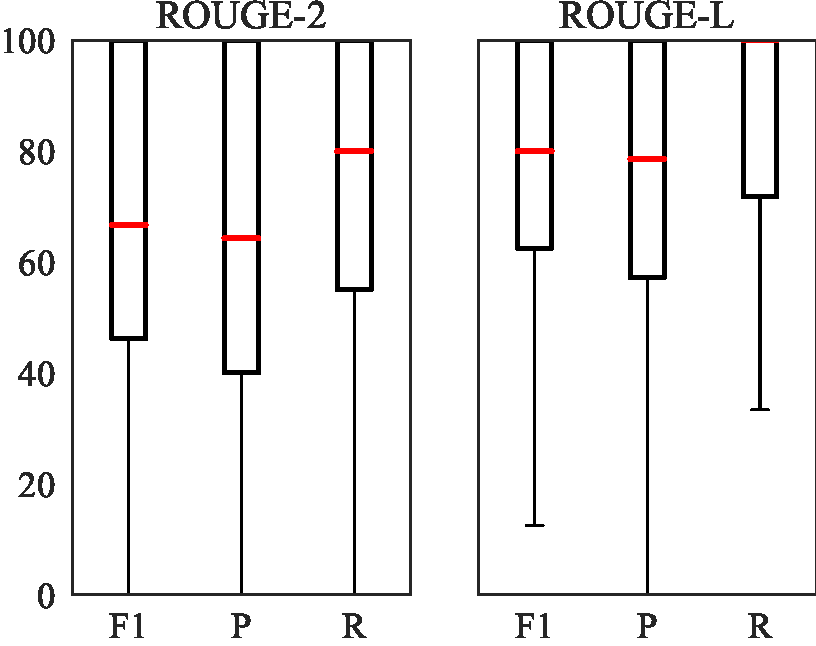
\includegraphics[width=.32\textwidth]{images/thesis/result_boxplots/logsummary_bart-large-cnn}}%
\hfill{}%
\subfloat[\bart{-XSum}]{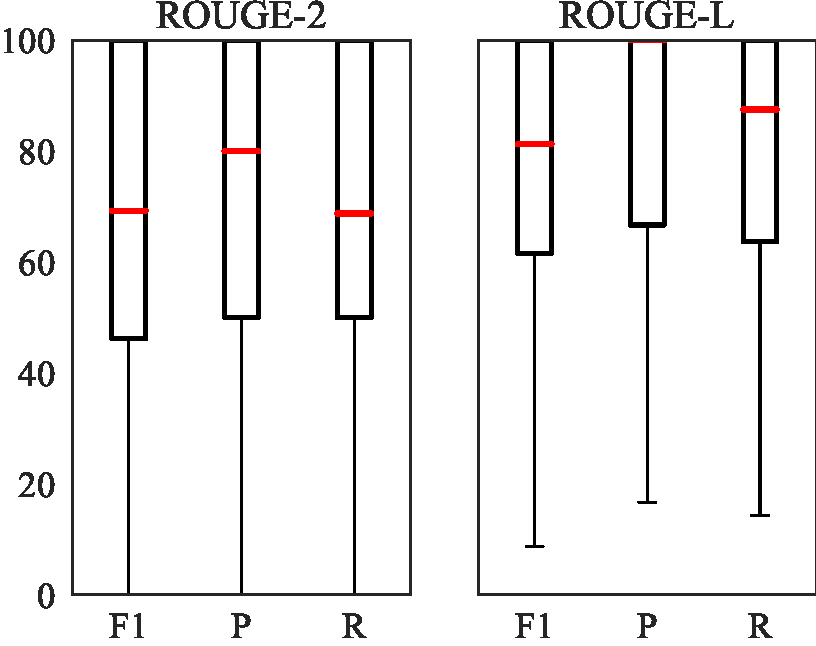
\includegraphics[width=.32\textwidth]{images/thesis/result_boxplots/logsummary_bart-large-xsum}}
\caption{Boxplots showing \acs*{rouge} recall, precision and \(F_1\)-scores
for different BART variants that have been further fine-tuned (\acs*{fsl}) on the \logsummary{} dataset.}
\label{fig:bart_trial_fsl_logsummary}
\end{figure}

In addition, we decide to qualitatively evaluate a summary generated in a \ac{zsl} setting,
and compare it to a summary written after fine-tuning.
To determine the models ability to select the log messages deemed relevant by the human-written reference,
we choose an example whose \ac{zsl}-prediction scores nearest to the median of
summary-level \acs*{rouge}-L recall on the \emph{Spark}-subdataset of \logsummary{}.
The precision would also measure the summary's conciseness, hence why we decide against using the \(F_1\)-score in this case.
We show the input, human-written summary
and \bart{-CNN}'s predictions in \autoref{tab:logsummary_bart_cnn_example}.
\bart{-CNN} is the BART-model that performed best in a \ac{zsl} setting according to perplexity.
For the \ac{zsl}-prediction we highlight the portions of the generated summary that correspond to the reference.

\begin{table}[htbp]
\centering
\footnotesize
%\setlength{\parskip}{0pt}\setlength{\parindent}{-1em}\setlength{\leftskip}{1em}
\begin{tabularx}{\textwidth}{>{\ttfamily\hbadness=10000}X>{\ttfamily\hbadness=10000}p{.2\textwidth}}
\toprule
\normalfont\textbf{input}
&\normalfont\textbf{reference summary}\\
\midrule
\tiny
Block rdd stored as bytes in memory ( estimated size 16.0 B , free 6.2 MB )

Block rdd stored as bytes in memory ( estimated size 16.0 B , free 6.2 MB )

Times : total = 38 , boot = 16 , init = 22 , finish = 0

Times : total = 37 , boot = 20 , init = 17 , finish = 0

Times : total = 38 , boot = 16 , init = 22 , finish = 0

Times : total = 38 , boot = 16 , init = 22 , finish = 0

Times : total = 38 , boot = 21 , init = 17 , finish = 0

Finished task 14.0 in stage 1359.0 ( TID 54654 ) . 2667 bytes result sent to driver

\textelp{} \textit{(4 similar messages discarded in this example for brevity)}

Got assigned task 54656

Running task 15.0 in stage 1359.0 ( TID 54656 )

\textelp{} \textit{(3 similar messages discarded in this example for brevity)}
&
\tiny
Running task

Finished task

Got assigned task

Block stored in memory
\\
\midrule
\normalfont\textbf{\bart{-CNN} \acs{zsl}}
&\normalfont\textbf{\bart{-CNN} \acs{fsl}}\\
\normalfont\tiny\acs*{rouge}-L recall: \(54.54\)
&\normalfont\tiny\acs*{rouge}-L recall: \(100\)\\
\midrule
\tiny
\h{\emph{Block}} rdd \h{\emph{stored}} as bytes \h{\emph{in memory}} ( estimated size 16.0 B, free 6.2 MB )

Times : total = 38, boot = 16, init = 22, finish = 0

\h{\emph{Finished task}} 14.0 in stage 1359.0 ( TID 54654 ). 2667 bytes result sent to driver
&
\tiny
Block stored in memory

Finished task

Running task

Got assigned task
\\
\bottomrule
\end{tabularx}
\caption{Representative predictions on an example from the \emph{Spark}-subdataset of \logsummary{}.}
\label{tab:logsummary_bart_cnn_example}
\end{table}

The example in \autoref{tab:logsummary_bart_cnn_example} shows that the model
quickly adapts to the style of the reference summaries in the \ac{fsl} setting.
For this example in particular it is able to extract the same text segments as the human-written reference,
albeit in a different order.

In the \ac{zsl} setting, the model correctly extracts some of the relevant log messages,
however it does not simplify them in any way, leading to a longer summary.
This is how we would want the model to behave on our other two datasets anyways,
but here this partly explains why model-generated summaries in the \ac{zsl} setting do not perform
as well concerning \acs*{rouge} precision and indirectly \(F_1\)-scores as in the \ac{fsl} setting.

Nevertheless, the model also performs worse in recall;
selecting a log message not considered important by the reference summary,
and missing two segments that were considered relevant.
This is a trend we can also observe when comparing the overall model performance from
\autoref{fig:bart_trial_zsl_logsummary} to \autoref{fig:bart_trial_fsl_logsummary}:
\bart{-CNN} performs much better regarding recall after fine-tuning.

Evidently all model variants perform significantly better concerning the overall \(F_1\)-scores after fine-tuning with a few examples.
As we saw significant improvements in model perplexity, this was to be expected.
Interestingly, on the \logsummary{} dataset this is mostly caused by a boost in precision,
as recall was high even before further fine-tuning.
As noted before, this jump in precision performance can be explained by the models' success in replicating
the condensed style of the human-written summaries.

In the \ac{zsl} setting we can roughly see that the \bart{-CNN} model performs best,
which matches up with the observed perplexities,
although the magnitude of differences between variants seem much less drastic.

Yet, the perplexities do not necessarily agree with the observed performance in the \ac{fsl} setting,
where \bart{-Large} shows the overall least reliable \(F_1\)-scores despite scoring first in perplexity.
Furthermore, the difference between the models seems to be mostly a trade-off between precision and recall,
as the median \(F_1\)-scores mostly match up:
\bart{-XSum} performs best at precision,
hinting at its ability to extract the most valuable information from each log message,
while \bart{-CNN} excels at recall.

Furthermore, we notice that model perplexity is also not comparable between different datasets,
as \ac{fsl} models perform better on the \logsummary{}-dataset than the \hadoop{}-dataset,
but perplexities on the \hadoop{}-dataset are low compared the perplexity of the same models fine-tuned on \logsummary{}.

Overall, these results affirm our verdict
that after training on a few examples,
models previously fine-tuned for summarization do not perform significantly
better on our summarization datasets
than their baselines.

We decide to select the \bart{-CNN} model for further evaluation,
as its recall values are highest,
which we take as an indicator that it manages to identify the most relevant log messages more reliably than the other the other two variants.

\subsection{Final Results on Summarization Capabilities}

Finally, we choose \bart{-CNN} and \pegasus{-Large} for thorough evaluation on all our datasets,
a decision which we motivated in the previous section.

We perform a hyperparameter search comprising 20 trials for each model on a validation set for every dataset
to determine an optimal length penalty for the beam-search.
Additionally for the \hadoop{}-dataset,
we disable the removal of duplicated trigrams of the beam-search for \bart{-CNN} used in the original implementation~\parencite[7876]{bart}:
The summaries in this dataset may contain many duplicated text segments,
and prohibiting the model from generating such duplicate sequences will drastically limit its performance.

The mean \(F_1\)-scores for \acs*{rouge}-1 to \acs*{rouge}-4
as well as sentence-level \acs*{rouge}-L and summary-level \acs*{rouge}-L
are reported in \autoref{tab:final_models_comparison} on \autopageref{tab:final_models_comparison} for the \ac{fsl} scenario
with the best results being highlighted.

As summaries in all our datasets are purely extractive,
and solely include text segments that are also present in the input data,
we should keep in mind that a \enquote{perfect} extractive model would be able to achieve
a score of \(100\) on every \acs*{rouge}-metric.

A more detailed analysis of each models performance is made in the following two segments.

\paragraph{BART}

We examine the summarization capabilities in a \ac{zsl} setting
and visualize the \acs*{rouge}-2 and summary-level \acs*{rouge}-L recall, precision and \(F_1\)-scores
in \autoref{fig:bart_cnn_zsl_all_datasets} for \bart{-CNN}.
For \ac{fsl} the results are shown in \autoref{fig:bart_cnn_fsl_all_datasets}.

\begin{figure}[htbp]
\centering
\subfloat[\logsummary{}]{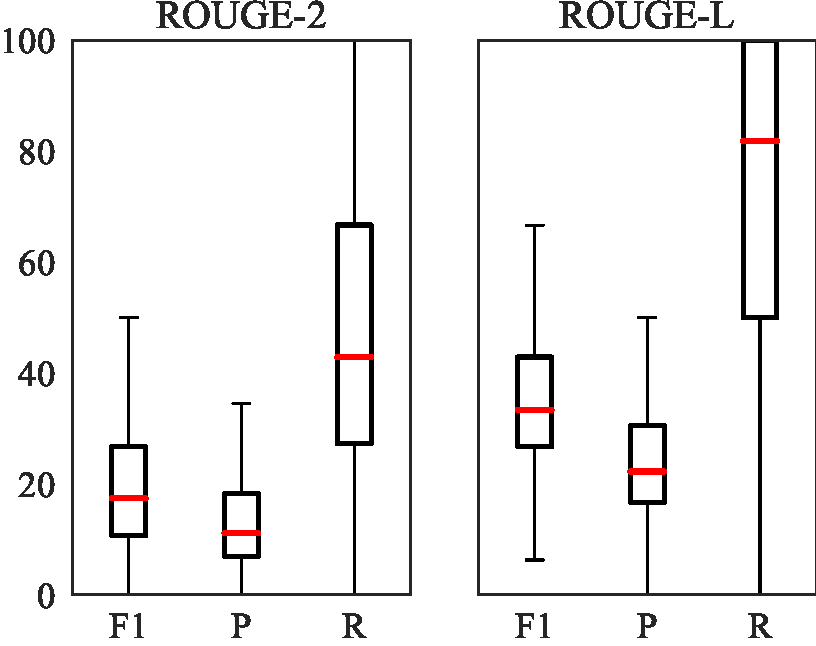
\includegraphics[width=.32\textwidth]{images/thesis/result_boxplots/logsummary_bart-large-cnn-zsl}}%
\hfill{}%
\subfloat[\hadoop{}]{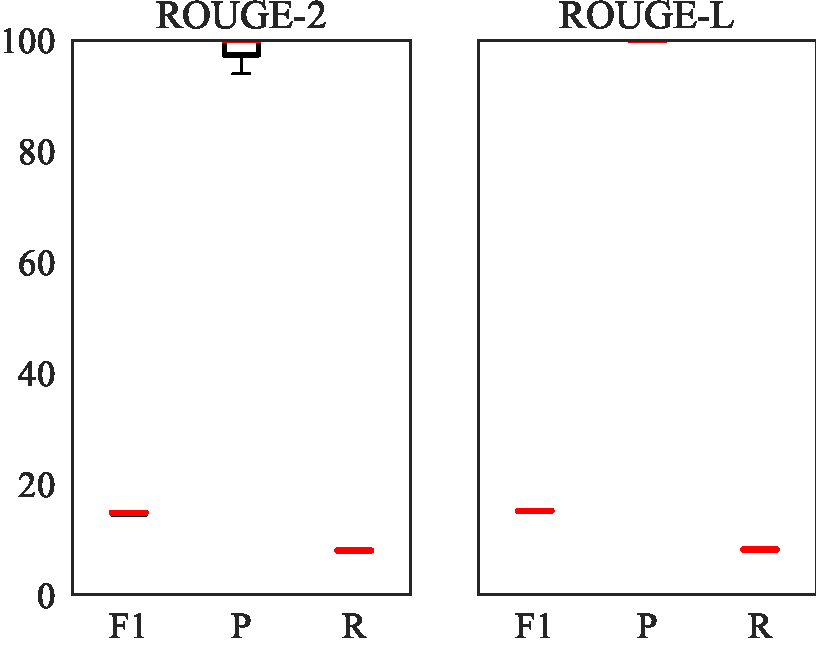
\includegraphics[width=.32\textwidth]{images/thesis/result_boxplots/hadoop_bart-large-cnn-zsl}}%
\hfill{}%
\subfloat[\telco{}]{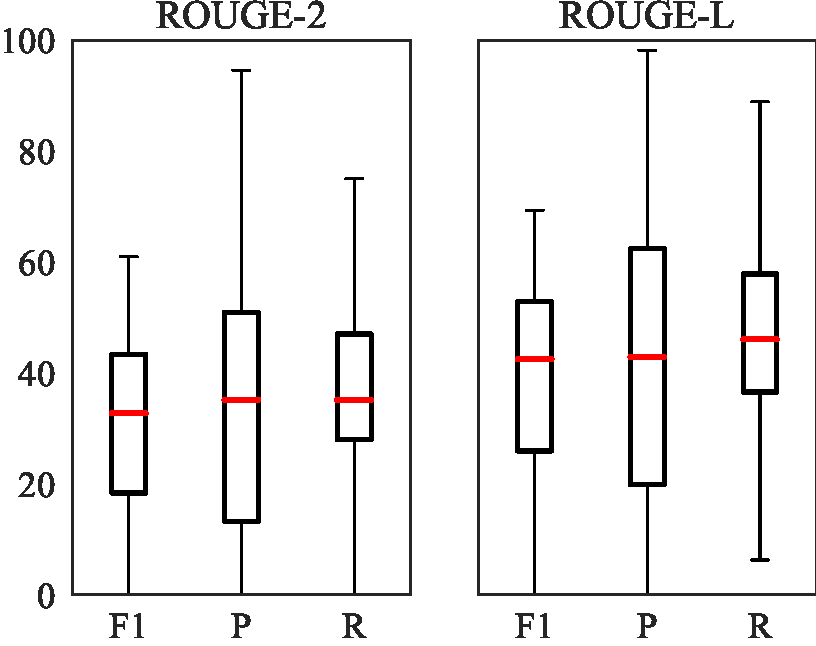
\includegraphics[width=.32\textwidth]{images/thesis/result_boxplots/telcoapp_bart-large-cnn-zsl}}
\caption{Boxplots showing \acs*{rouge} recall, precision and \(F_1\)-scores
of \bart{-CNN} without further fine-tuning (\acs*{zsl}) on all datasets.}
\label{fig:bart_cnn_zsl_all_datasets}
\end{figure}

\begin{figure}[htbp]
\centering
\subfloat[\logsummary{}]{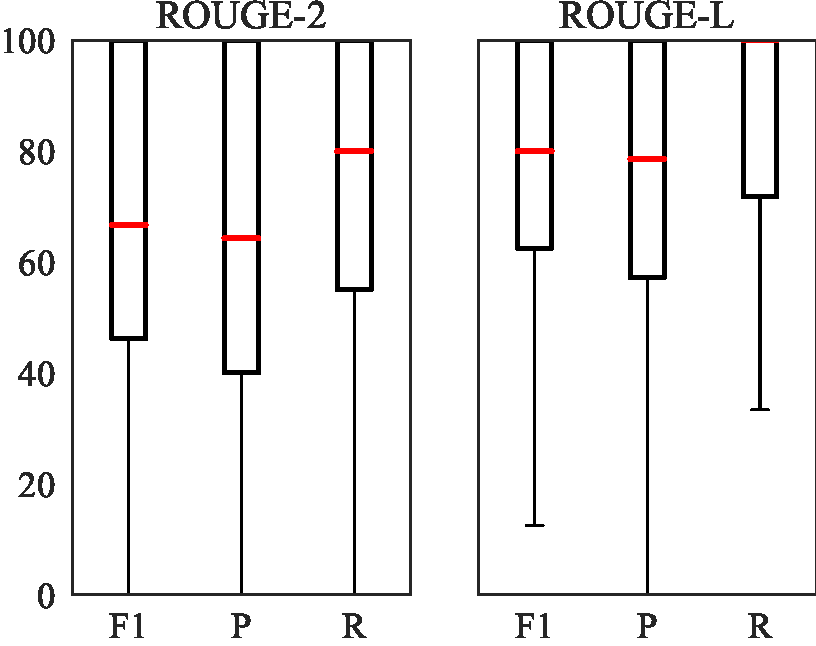
\includegraphics[width=.32\textwidth]{images/thesis/result_boxplots/logsummary_bart-large-cnn}}%
\hfill{}%
\subfloat[\hadoop{}]{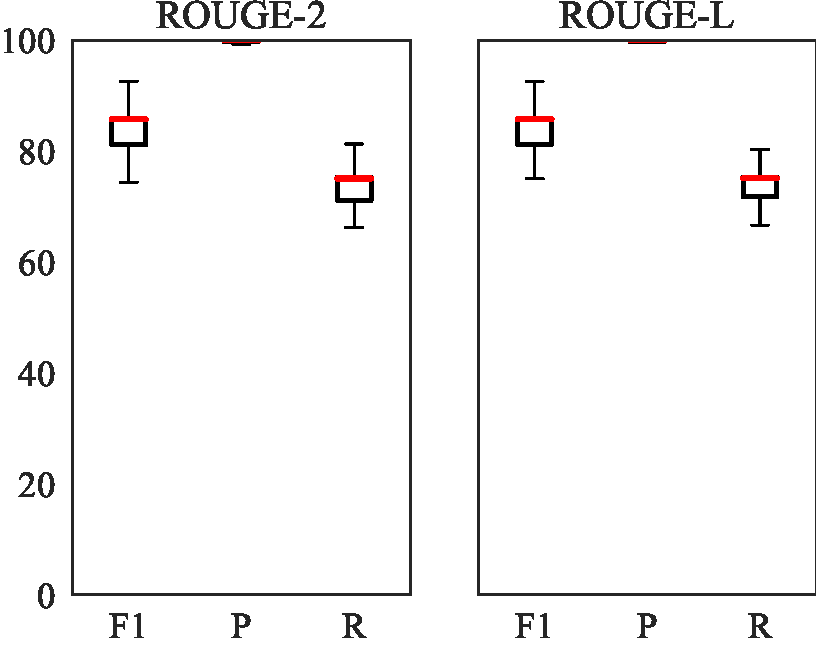
\includegraphics[width=.32\textwidth]{images/thesis/result_boxplots/hadoop_bart-large-cnn}}%
\hfill{}%
\subfloat[\telco{}]{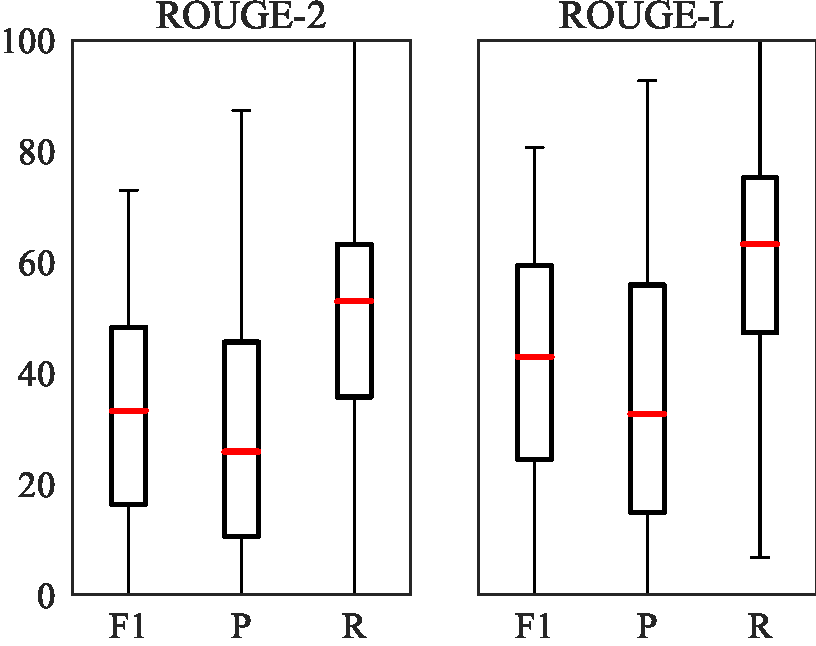
\includegraphics[width=.32\textwidth]{images/thesis/result_boxplots/telcoapp_bart-large-cnn}}
\caption{Boxplots showing \acs*{rouge} recall, precision and \(F_1\)-scores
of \bart{-CNN} with further fine-tuning (\acs*{fsl}) on all datasets.}
\label{fig:bart_cnn_fsl_all_datasets}
\end{figure}

While we previously found that fine-tuning improves performance substantially,
this seems less clear when looking at the BART-model's performance on the \telco{}-dataset.
The \(F_1\) scores remained at almost the same level, though recall is noticeably higher;
at the expense of a equally lower precision.
Unfortunately, it seems that fine-tuning was not able to improve the performance on this dataset,
though it should be noted that the model was able to extract \(49.4\%\)
of the information contained in the reference summary \emph{without} any fine-tuning,
according to the mean summary-level \acs*{rouge}-L recall.
This is while keeping around \(42.3\%\) of the information in the summary relevant,
according to the mean summary-level \acs*{rouge}-L precision.

We do observe however strict improvements on the \hadoop{} and \logsummary{} datasets,
on \hadoop{} mostly due to a substantial improvement in recall.
The results on both datasets seem promising.

However, the \hadoop{}-dataset is actually comprised of logs from 3 failure types,
which are not present in equal proportions, while running one of two different applications.
As the summaries vary in length and form between failure types,
it becomes important to also consider the results for each failure separately.
Thus we report the same metrics as before
in \autoref{fig:bart_cnn_zsl_all_datasets} for  the \ac{zsl} case,
and in \autoref{fig:bart_cnn_fsl_all_datasets} for \ac{fsl}.

\begin{figure}[b]
\centering
\subfloat[Disk full\\\,\clap{\scriptsize{}(15 examples)}]{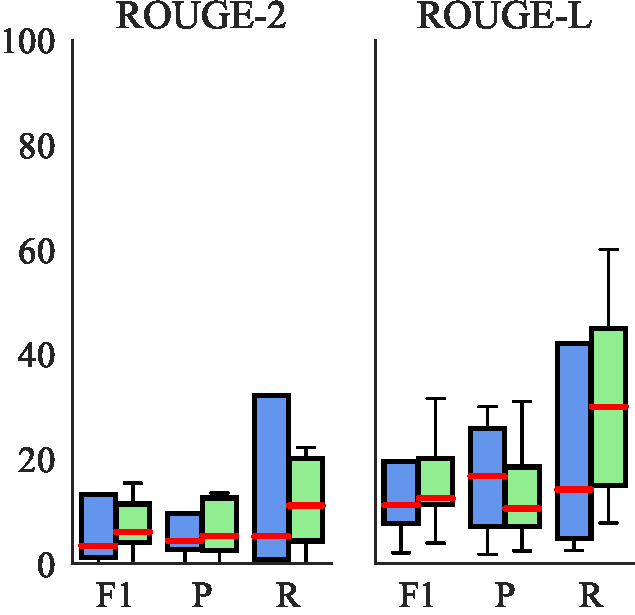
\includegraphics[width=.32\textwidth]{images/thesis/result_boxplots/bart-large-cnn-zsl_disk_full}}%
\hfill{}%
\subfloat[Machine down\\\,\clap{\scriptsize{}(214 examples)}]{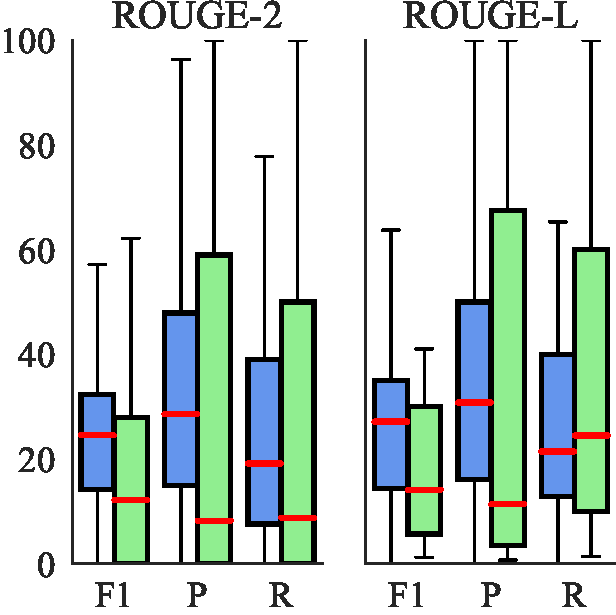
\includegraphics[width=.32\textwidth]{images/thesis/result_boxplots/bart-large-cnn-zsl_machine_down}}%
\hfill{}%
\subfloat[Network disconnection\\\,\clap{\scriptsize (826 examples)}]{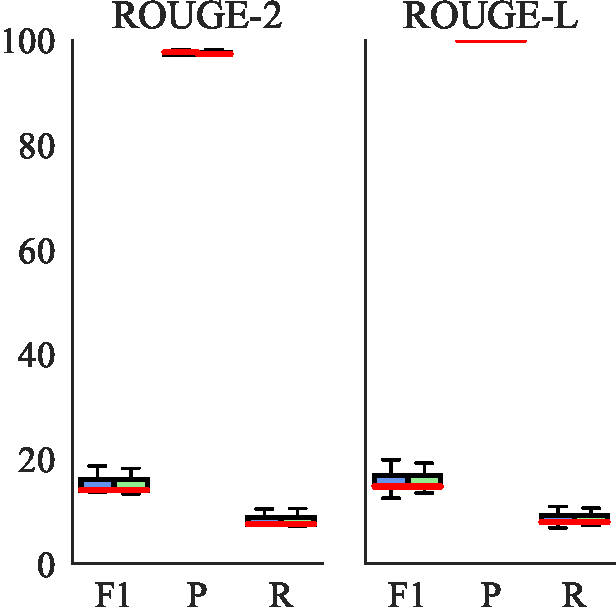
\includegraphics[width=.32\textwidth]{images/thesis/result_boxplots/bart-large-cnn-zsl_network_disconnection}}
\caption[Boxplots showing \acs*{rouge} recall, precision and \(F_1\)-scores
of \bart{-CNN} without further fine-tuning (\acs*{zsl}) on \hadoop{} categorized by failure type and application.]{Boxplots showing \acs*{rouge} recall, precision and \(F_1\)-scores
of \bart{-CNN} without further fine-tuning (\acs*{zsl}) on \hadoop{} categorized by failure type and application (PageRank on the left, WordCount on the right).}
\label{fig:bart_cnn_zsl_hadoop}
\end{figure}

\begin{figure}[t]
\centering
\subfloat[Disk full\\\,\clap{\scriptsize{}(15 examples)}]{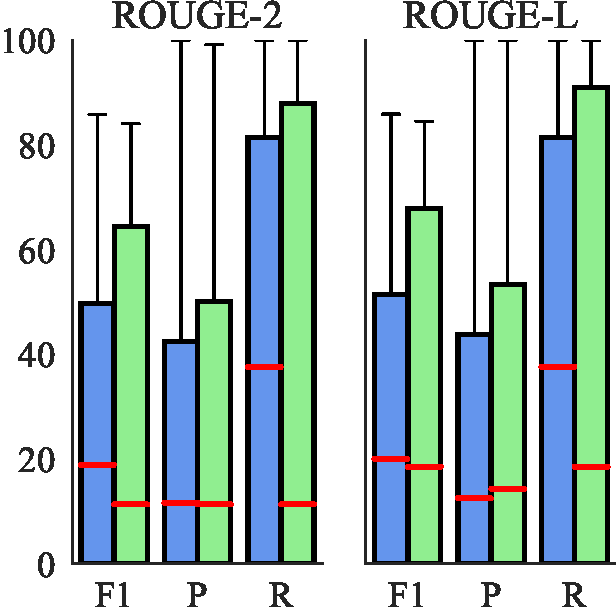
\includegraphics[width=.32\textwidth]{images/thesis/result_boxplots/bart-large-cnn_disk_full}}%
\hfill{}%
\subfloat[Machine down\\\,\clap{\scriptsize{}(214 examples)}]{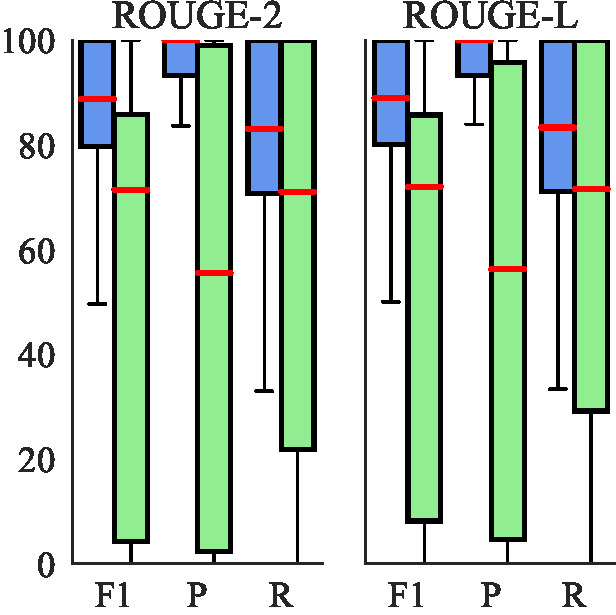
\includegraphics[width=.32\textwidth]{images/thesis/result_boxplots/bart-large-cnn_machine_down}}%
\hfill{}%
\subfloat[Network disconnection\\\,\clap{\scriptsize{}(826 examples)}]{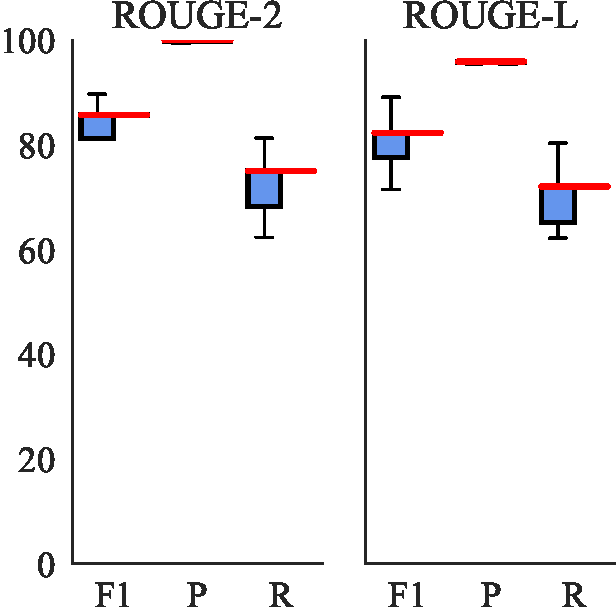
\includegraphics[width=.32\textwidth]{images/thesis/result_boxplots/bart-large-cnn_network_disconnection}}
\caption[Boxplots showing \acs*{rouge} recall, precision and \(F_1\)-scores
of \bart{-CNN} with further fine-tuning (\acs*{fsl}) on \hadoop{} categorized by failure type and application.]{Boxplots showing \acs*{rouge} recall, precision and \(F_1\)-scores
of \bart{-CNN} with further fine-tuning (\acs*{fsl}) on \hadoop{} categorized by failure type and application (PageRank on the left, WordCount on the right).}
\label{fig:bart_cnn_fsl_all_hadoop}
\end{figure}

Now we can see that the \hadoop{}-dataset includes mostly examples from a \emph{network disconnection} failure,
which overshadow the results on the two other failure types.
The continued fine-tuning improved precision \emph{and} recall,
except for the \emph{full disk} failure type where the continued training actually decreased the precision or recall in some cases.

It should be reiterated,
that the training set contained 5 examples for each application on the \emph{full disk} failure,
leaving 11 examples from the WordCount application
and 4 examples from the PageRank application in the test set for this failure type.
Hence we might expect the models to do best in the \ac{fsl} setting here,
as it has trained with a higher proportion of the available examples compared to the other to failure types.
However this is not at all what we observe:
Both precision and recall vary widely and especially for the WordCount application little improvements could be made.
It is not empirically sound to take conclusions concerning the performance difference between the applications on this failure type
due to the imbalanced and low number of test examples available for each application.

An evaluation of the performance on the \emph{machine down} failure is more meaningful,
as the model has only seen 10 examples per application in this dataset.
The test set then contains 181 examples for PageRank and 33 for WordCount.
Again, this is quite imbalanced between applications,
hence why we might expect the model to do better on the WordCount application,
where it has been trained on a greater share of examples.
Instead we observe that the model maintains its preference for the PageRank summaries from the \ac{zsl}-phase.

Regarding this same failure,
for PageRank the model's summaries actually include \(81.1\%\) of the tokens contained in the non-normal log messages
according to the mean summary-level \acs*{rouge}-L recall after pre-training.
On the other hand, the summaries contain \(16.7\%\) tokens not present in the reference summaries
according to the complement of the mean summary-level \acs*{rouge}-L precision.
As such, the model does manage to identify over \(\frac{4}{5}\) of the relevant information,
while keeping the amount of irrelevant information close to \(\frac{1}{6}\).

Though, one-sixth of \emph{factually inconsistent} information
would still be harmful to the quality of the summaries.
Unfortunately \acs*{rouge} is unable to judge the origin or truthiness of the irrelevant portions of the summary.
As such, and to further gain an intuitive understanding of the big variance in performance between the failure types,
we also qualitatively examine one representative example for each failure.

We choose an example whose \ac{fsl}-prediction scores nearest to the median of
summary-level \acs*{rouge}-L \(F_1\) score for each failure type,
to get an idea of the model's average summarization ability.
For comparison we also show the summary in the \ac{zsl} setting,
but omit the input to the model for brevity.

The results are shown in
\autoref{tab:bart_cnn_hadoop_disk_full_example} for the \emph{full disk} failure,
\autoref{tab:bart_cnn_hadoop_machine_down_example} for the \emph{machine down} failure,
and
\autoref{tab:bart_cnn_hadoop_network_disconnection_example} for the \emph{network disconnection} failure.

\begin{table}[htbp]
\centering
\footnotesize
\setlength{\parskip}{1cm}
\begin{tabularx}{\textwidth}{XXX}
\toprule
\textbf{reference summary}
&\textbf{\bart{-CNN} \ac{fsl}}
&\textbf{\bart{-CNN} \ac{zsl}}\\
&\tiny\acs*{rouge}-L \(F_1\): \(18.52\)
&\tiny\acs*{rouge}-L \(F_1\): \(11.88\)\\
\midrule
\tiny\ttfamily\hbadness=10000
Task: attempt\#59489 - exited : DiskChecker: Could not find any valid local directory for out-path

Diagnostics report from attempt\#59489: Error: DiskChecker: Could not find any valid local directory for out-path

Diagnostics report from attempt\#59489: Error: DiskChecker: Could not find any valid local directory for out-path

1 failures on node microsoft.
&
\tiny\ttfamily\hbadness=10000
Diagnostics report from attempt\#83820: Container killed by the ApplicationMaster. Container killed on request. Exit code is 137 Container exited with a non-zero exit code 137

Diagnostics report from attempt\#97248: Container killed by the ApplicationMaster. Container killed on request. Exit code is 137 Container exited with a non-zero exit code 137
&
\tiny\ttfamily\hbadness=10000
Diagnostics report from attempt\#83820: Container killed by the ApplicationMaster. Exit code is 137 Container exited with a non-zero exit code 137. After Scheduling: PendingReds:0 ScheduledMaps:0 ScheduledReds:0 AssignedMaps:3 AssignedReds:1 CompletedMaps:8 CompletedReds:0 ContAlloc:19 ContRel:0 HostLocal:10 RackLocal:8.
\\
\bottomrule
\end{tabularx}
\caption{Representative predictions on a full disk failure of \hadoop{}.}
\label{tab:bart_cnn_hadoop_disk_full_example}
\end{table}

\begin{table}[htbp]
\centering
\footnotesize
\setlength{\parskip}{1cm}
\begin{tabularx}{\textwidth}{XXX}
\toprule
\textbf{reference summary}
&\textbf{\bart{-CNN} \ac{fsl}}
&\textbf{\bart{-CNN} \ac{zsl}}\\
&\tiny\acs*{rouge}-L \(F_1\): \(88.89\)
&\tiny\acs*{rouge}-L \(F_1\): \(22.43\)\\
\midrule
\tiny\ttfamily\hbadness=10000
Retrying connect to server: microsoft. Already tried 15 time(s); maxRetries=45

\textelp{} \textit{(message repeats 4 times with different retry-counts)}
&
\tiny\ttfamily\hbadness=10000
Retrying connect to server: microsoft. Already tried 15 time(s)

maxRetries=45

\textelp{} \textit{(messages repeat 3 times with different retry-counts)}
&
\tiny\ttfamily\hbadness=10000
Retrying connect to server: microsoft. Already tried 15 time(s)

maxRetries=45

Progress of TaskAttempt attempt\#14835 is : 0.23333333

MapCompletionEvents request from attempt\#14835. startIndex 7 maxEvents 10000

\textelp{} \textit{(message repeats 2 times)}
\\
\bottomrule
\end{tabularx}
\caption{Representative predictions on a machine down failure of \hadoop{}.}
\label{tab:bart_cnn_hadoop_machine_down_example}
\end{table}

\begin{table}[htbp]
\centering
\footnotesize
\setlength{\parskip}{1cm}
\begin{tabularx}{\textwidth}{XXX}
\toprule
\textbf{reference summary}
&\textbf{\bart{-CNN} \ac{fsl}}
&\textbf{\bart{-CNN} \ac{zsl}}\\
&\tiny\acs*{rouge}-L \(F_1\): \(82.28\)
&\tiny\acs*{rouge}-L \(F_1\): \(15.09\)\\
\midrule
\tiny\ttfamily\hbadness=10000
Failed to renew lease for NONMAPREDUCE for 1389 seconds. Will retry shortly... NoRouteToHostException: No Route to Host from MININT-FNANLI5remote host \#73234 to msra-sa-41:9000 failed on socket timeout exception: NoRouteToHostException: No route to host: no further information; For more details see: http-URL Caused by: NoRouteToHostException: No route to host: no further information

Address change detected. Old: msra-sa-41remote host \#94343 New: msra-sa-41:9000

\textelp{} \textit{(messages repeat 6 times with incremented timeout)}
&
\tiny\ttfamily\hbadness=10000
Failed to renew lease for NONMAPREDUCE for 1389 seconds. Will retry shortly... NoRouteToHostException: No Route to Host from MININT-FNANLI5remote host \#73234 to msra-sa-41:9000 failed on socket timeout exception: NoRouteToHostException: No route to host: no further information

For more details see: http-URL Caused by: NoRouteToHostException: No route to host: no further information

Address change detected. Old: msra-sa-41remote host \#94343 New: msra-sa-41:9000

\textelp{} \textit{(messages repeat 4 times with incremented timeout)}

Failed to renew lease for NONMAPREDUCE for 1394 seconds. Will retry shortly... NoRouteToHostException: No Route to Host from
&
\tiny\ttfamily\hbadness=10000
Failed to renew lease for NONMAPREDUCE for 1389 seconds. Will retry shortly... NoRouteToHostException: No Route to Host from MININT-FNANLI5remote host \#73234 to msra-sa-41:9000 failed on socket timeout exception: NoRouteToHostException: No route to host: no further information.
\\
\bottomrule
\end{tabularx}
\caption{Representative predictions on a network disconnection failure of \hadoop{}.}
\label{tab:bart_cnn_hadoop_network_disconnection_example}
\end{table}

If we interpret the summaries for the full disk failure in \autoref{tab:bart_cnn_hadoop_disk_full_example},
we notice that the model has learned that messages starting with \verb+Diagnostics report from attempt+ usually are important.
Looking at the reference summary provided in that example, this does seem to be usually the case.
Unfortunately, in this specific case this heuristic did not work out for the model,
because the cancellation of an attempt is actually an benign activity,
and the model failed to include any of the more relevant messages about disk failures.

In the case of the machine down failure in \autoref{tab:bart_cnn_hadoop_network_disconnection_example},
the model missed to include one repetition of the relevant message and would have achieved a perfect score otherwise.

Similarly, for the network disconnection failure in \autoref{tab:bart_cnn_hadoop_network_disconnection_example}
we can actually speculate that the \ac{fsl} model would have correctly continued the message,
however it was cutoff by a maximum length limit we imposed upon the beam-search.
As this is the typical structure of a network disconnection failure,
we can expect that the recall would actually improve on this failure type,
if we had allowed the model to generate longer summaries.
As it maintained a close to perfect precision on this failure until now,
this would probably result in a strict improvement of \(F_1\) scores.

Overall, the model does well in the last two failure types,
where summaries often repeat a message multiple time,
but does worse for the more diverse full disk failure.
On the other hand, this is also where the model has experienced less training.

The \ac{zsl} model performs worse in all examples,
managing to select some of the same messages as the model in the \ac{fsl} setting,
but also including a great portion of irrelevant messages.

Yet, we have to wonder whether this success in caused by the models summarization abilities,
or if the summaries are just too trivial. For the network disconnection failure specifically,
the repeated message which is part of the summary is quite long.
As such they likely represent a majority of the input data.\\
We decide to investigate and calculate the ratio of log messages shared between the model inputs and the reference summaries,
visualizing the results in \autoref{fig:hadoop_summary_document_overlap}.

\begin{figure}[htbp]
\centering
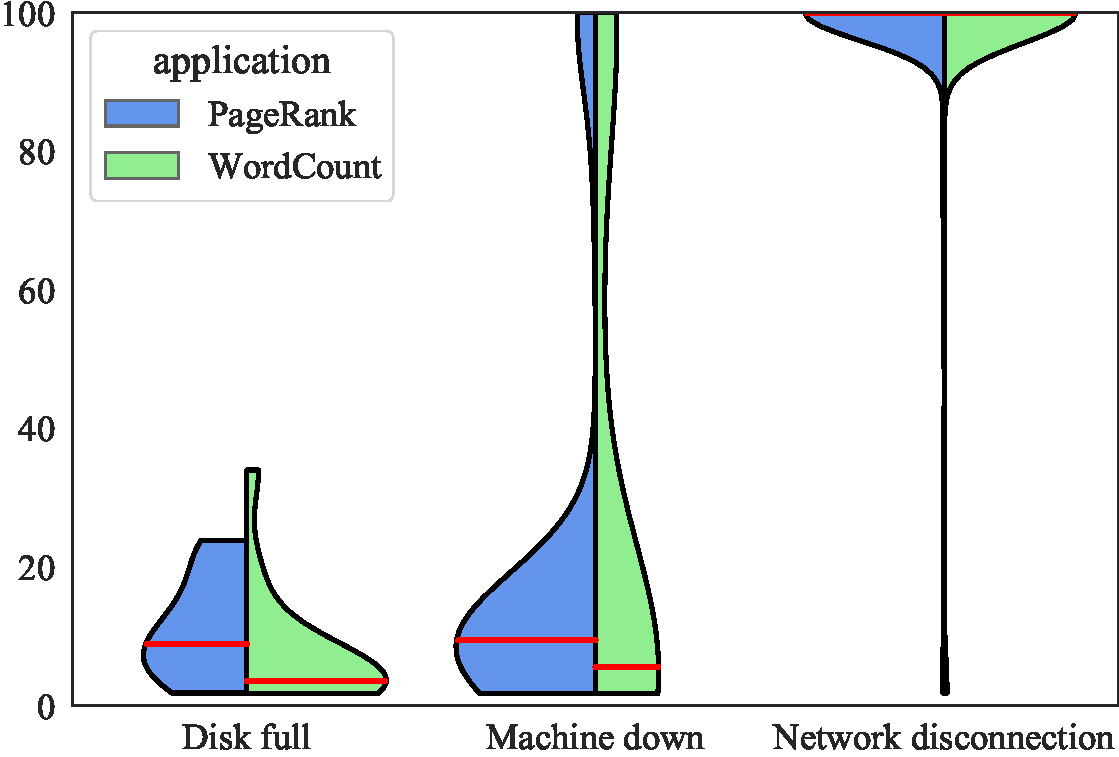
\includegraphics[width=.75\textwidth]{images/thesis/hadoop_curated_summary_document_overlap}
\caption{Violin plot showing the percentage of log messages shared between model inputs and the summaries on \hadoop{}.}
\label{fig:hadoop_summary_document_overlap}
\end{figure}

It is clear now that on the network disconnection failure we do not actually evaluate the model's performance to summarize,
since the input and reference summaries are identical in most cases.
Rather, the \ac{fsl} model as just learned to replicate the relevant message as many times as needed,
while the \ac{zsl} model just selects the first occurrence.
However, the summarization task is meaningful on the other two failure types.
Concerning the machine down failure type, we can now infer a cause for the difference in performance between the logs from the PageRank and WordCount applications:
As indicated by the higher median, the summaries for the PageRank application share more log messages with the input documents.
We assume this is one cause of the higher performance we observe for logs originating during the execution of the PageRank application.

All in all, the example predictions were factually consistent,
including only log messages present in the input data,
but sometimes selecting irrelevant ones.
From manually inspecting other examples,
we conclude that this is the situation in general.

\paragraph{PEGASUS}

Again, we visualize the \acs*{rouge}-2 and summary-level \acs*{rouge}-L recall, precision and \(F_1\)-scores
in \autoref{fig:pegasus_large_zsl_all_datasets} for \pegasus{-Large} under the \ac{zsl} setting.
For \ac{fsl} the results are shown in \autoref{fig:pegasus_large_fsl_all_datasets}.

\begin{figure}[p]
\centering
\subfloat[\logsummary{}]{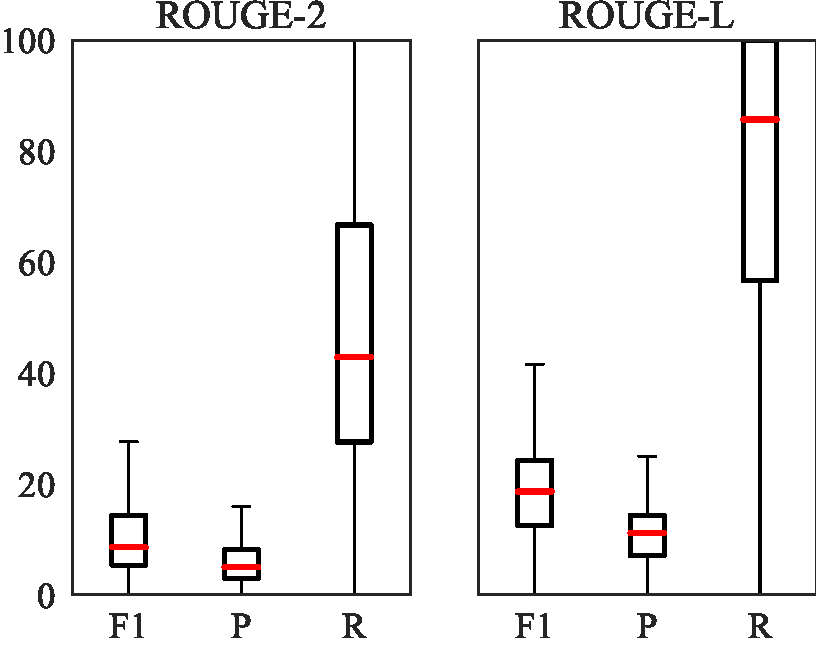
\includegraphics[width=.32\textwidth]{images/thesis/result_boxplots/logsummary_pegasus-large-zsl}}%
\hfill{}%
\subfloat[\hadoop{}]{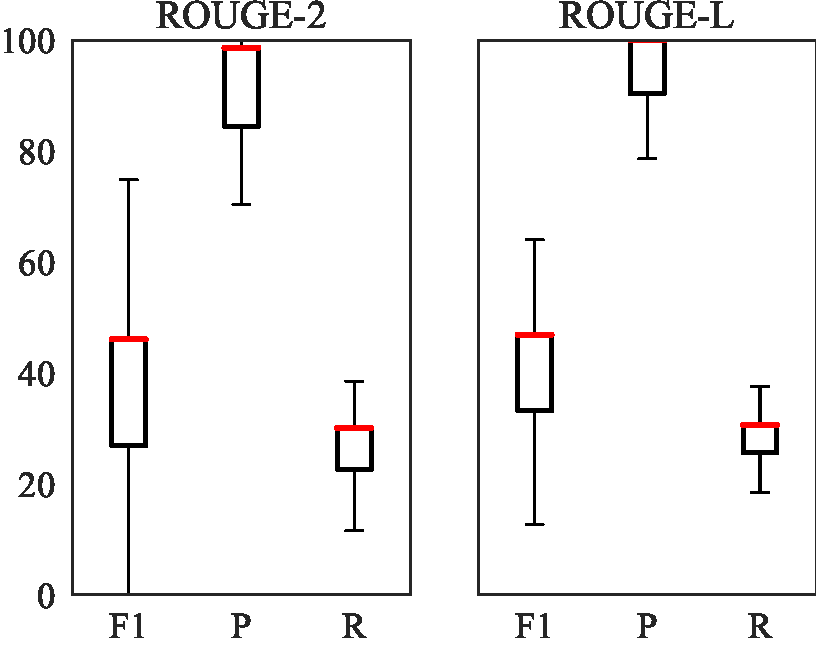
\includegraphics[width=.32\textwidth]{images/thesis/result_boxplots/hadoop_pegasus-large-zsl}}%
\hfill{}%
\subfloat[\telco{}]{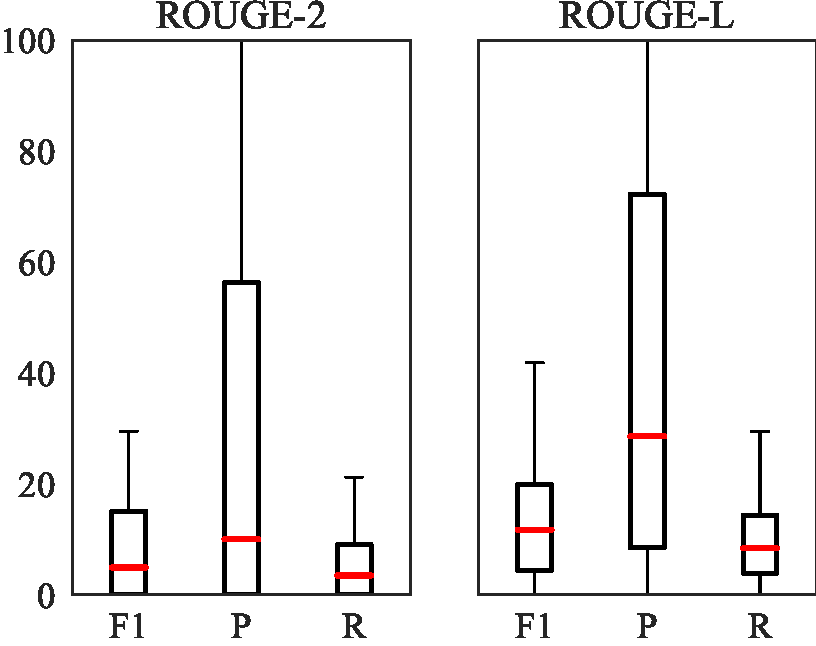
\includegraphics[width=.32\textwidth]{images/thesis/result_boxplots/telcoapp_pegasus-large-zsl}}
\caption{Boxplots showing \acs*{rouge} recall, precision and \(F_1\)-scores
of \pegasus{-Large} without further fine-tuning (\acs*{zsl}) on all datasets.}
\label{fig:pegasus_large_zsl_all_datasets}
\end{figure}

\begin{figure}[p]
\centering
\subfloat[\logsummary{}]{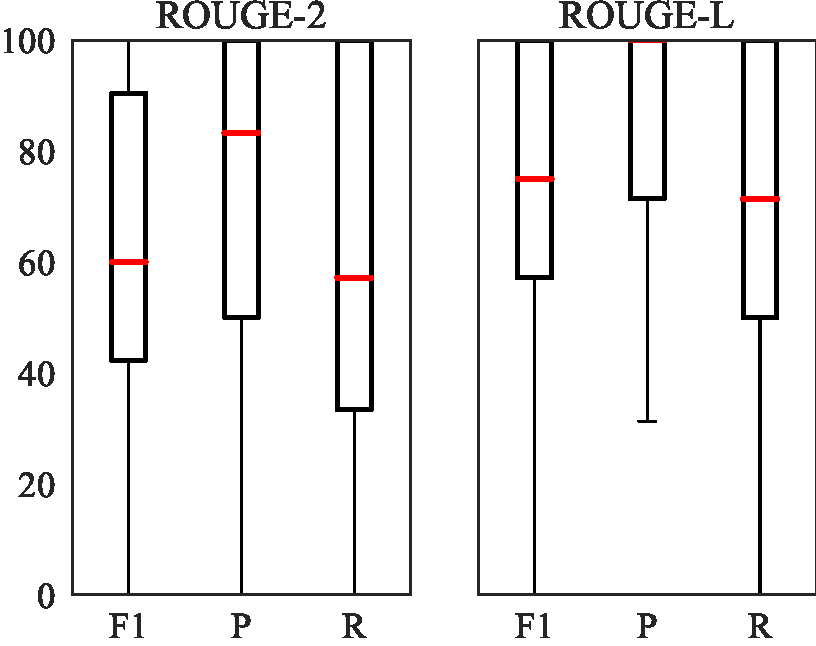
\includegraphics[width=.32\textwidth]{images/thesis/result_boxplots/logsummary_pegasus-large}}%
\hfill{}%
\subfloat[\hadoop{}]{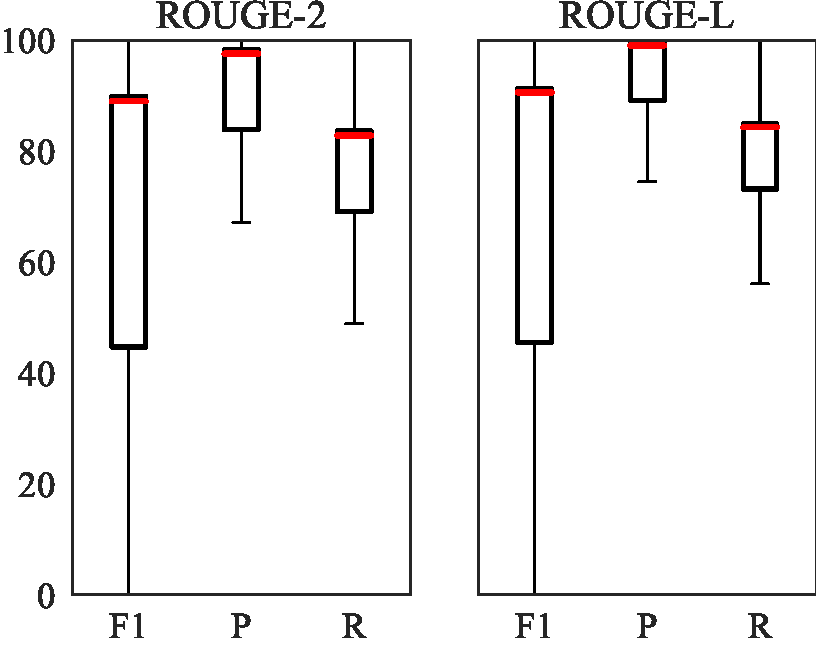
\includegraphics[width=.32\textwidth]{images/thesis/result_boxplots/hadoop_pegasus-large}}%
\hfill{}%
\subfloat[\telco{}]{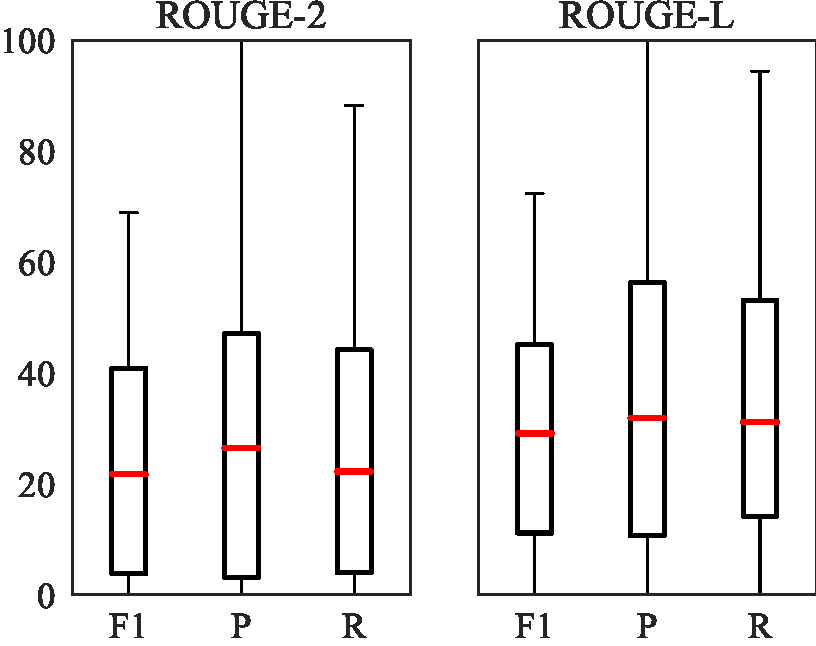
\includegraphics[width=.32\textwidth]{images/thesis/result_boxplots/telcoapp_pegasus-large}}
\caption{Boxplots showing \acs*{rouge} recall, precision and \(F_1\)-scores
of \pegasus{-Large} with further fine-tuning (\acs*{fsl}) on all datasets.}
\label{fig:pegasus_large_fsl_all_datasets}
\end{figure}

The fine-tuning for \pegasus{-Large} actually helped on all datasets, even on \telco{}.
However, one should point out that \bart{-CNN} performed more than twice as good in a \ac{zsl} setting
compared to \pegasus{-Large}, when considering the median \(F_1\)-score for summary-level \acs*{rouge}-L.
Even after fine-tuning this situation does not improve by much.

On the \telco{} dataset we observe that the PEGASUS model manages to achieve higher precision than the BART model in a \ac{fsl} setting,
at the expense of recall.

Finally, on the \hadoop{} dataset the achieved performances vary much more than with \bart{-CNN}.
This remains true when considering the results by failure type,
shown in \autoref{fig:pegasus_large_zsl_hadoop} for the \ac{zsl} case,
and in \autoref{fig:pegasus_large_fsl_hadoop} for \ac{fsl}.

\begin{figure}[htbp]
\centering
\subfloat[Disk full\\\,\clap{\scriptsize{}(15 examples)}]{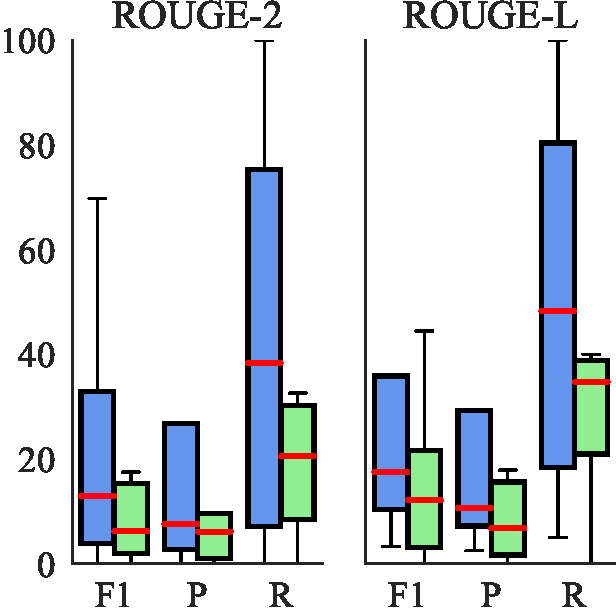
\includegraphics[width=.32\textwidth]{images/thesis/result_boxplots/pegasus-large-zsl_disk_full}}%
\hfill{}%
\subfloat[Machine down\\\,\clap{\scriptsize{}(214 examples)}]{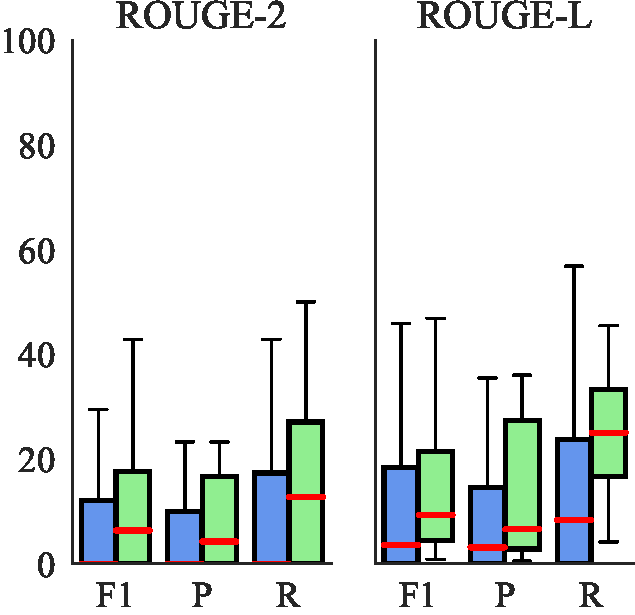
\includegraphics[width=.32\textwidth]{images/thesis/result_boxplots/pegasus-large-zsl_machine_down}}%
\hfill{}%
\subfloat[Network disconnection\\\,\clap{\scriptsize (826 examples)}]{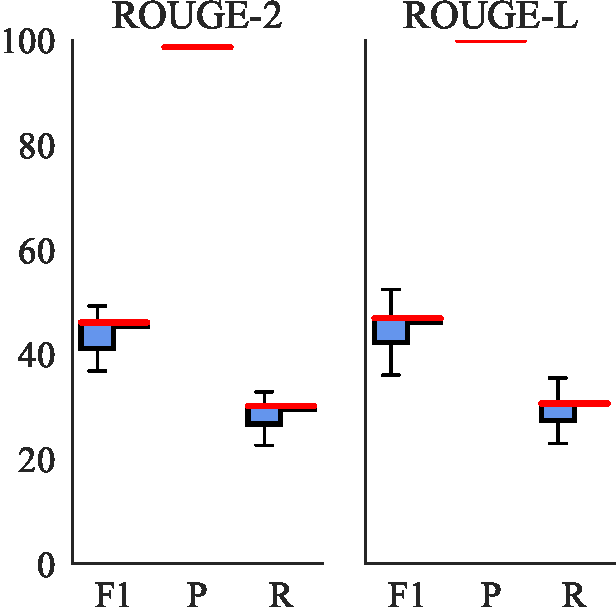
\includegraphics[width=.32\textwidth]{images/thesis/result_boxplots/pegasus-large-zsl_network_disconnection}}
\caption[Boxplots showing \acs*{rouge} recall, precision and \(F_1\)-scores
of \pegasus{-Large} without further fine-tuning (\acs*{zsl}) on \hadoop{} categorized by failure type and application.]{Boxplots showing \acs*{rouge} recall, precision and \(F_1\)-scores
of \pegasus{-Large} without further fine-tuning (\acs*{zsl}) on \hadoop{} categorized by failure type and application (PageRank on the left, WordCount on the right).}
\label{fig:pegasus_large_zsl_hadoop}
\end{figure}

\begin{figure}[htbp]
\centering
\subfloat[Disk full\\\,\clap{\scriptsize{}(15 examples)}]{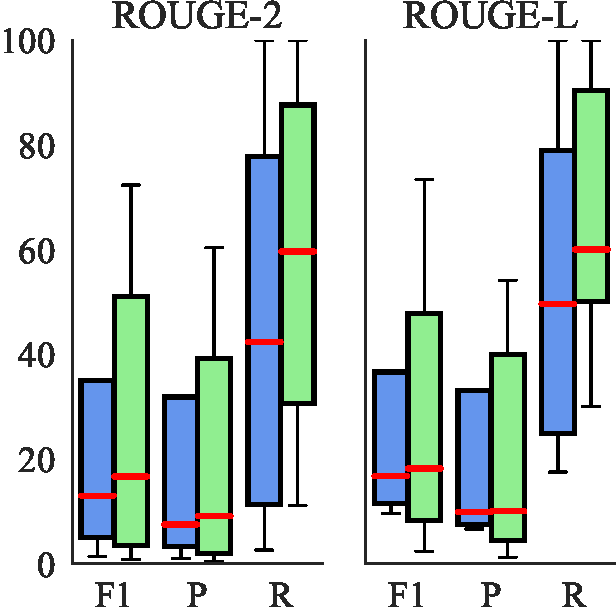
\includegraphics[width=.32\textwidth]{images/thesis/result_boxplots/pegasus-large_disk_full}}%
\hfill{}%
\subfloat[Machine down\\\,\clap{\scriptsize{}(214 examples)}]{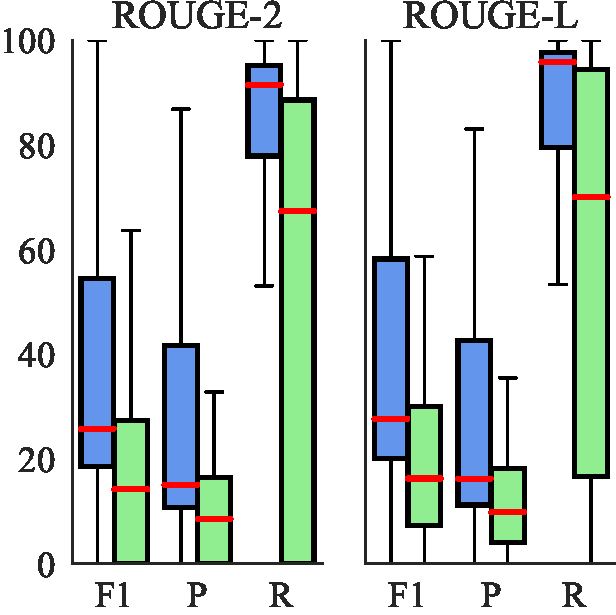
\includegraphics[width=.32\textwidth]{images/thesis/result_boxplots/pegasus-large_machine_down}}%
\hfill{}%
\subfloat[Network disconnection\\\,\clap{\scriptsize{}(826 examples)}]{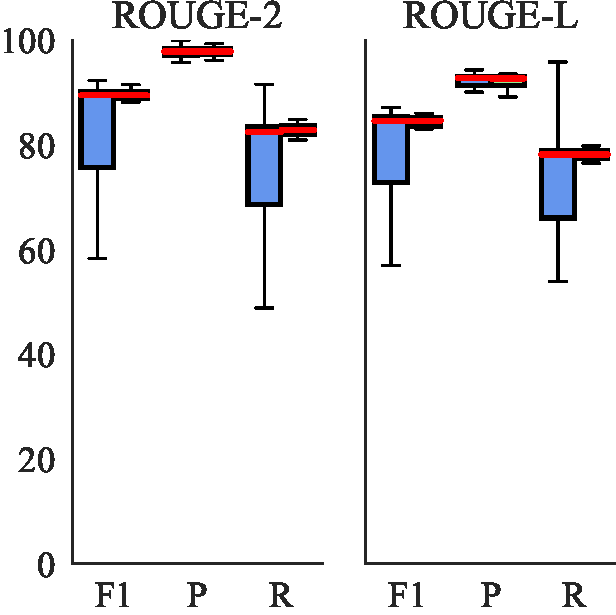
\includegraphics[width=.32\textwidth]{images/thesis/result_boxplots/pegasus-large_network_disconnection}}
\caption[Boxplots showing \acs*{rouge} recall, precision and \(F_1\)-scores
of \pegasus{-Large} with further fine-tuning (\acs*{fsl}) on \hadoop{} categorized by failure type and application.]{Boxplots showing \acs*{rouge} recall, precision and \(F_1\)-scores
of \pegasus{-Large} with further fine-tuning (\acs*{fsl}) on \hadoop{} categorized by failure type and application (PageRank on the left, WordCount on the right).}
\label{fig:pegasus_large_fsl_hadoop}
\end{figure}

Altogether,
\bart{-CNN} outperforms \pegasus{-Large} in all observed settings as can be seen in \autoref{tab:final_models_comparison},
where the best results have been highlighted.
As such we decide to omit any further investigations of the performance of the PEGASUS model for the sake of brevity.

\begin{table}[htbp]
\centering
\footnotesize
\begin{tabular}{rccc}
                          & \multicolumn{3}{c}{\scriptsize{}\bart{-CNN} / \pegasus{-Large}}\\
                          & \h{\logsummary{}}       & \h{\hadoop{}}           & \h{\telco{}}\\
\midrule
\acs*{rouge}-1            & \h{76.3}/72.9           & \h{75.8}/70.4           & \h{40.5}/29.6\\
\acs*{rouge}-2            & \h{66.0}/61.7           & \h{75.6}/68.5           & \h{33.0}/23.7\\
\acs*{rouge}-3            & \h{52.8}/45.9           & \h{75.4}/66.9           & \h{29.2}/21.5\\
\acs*{rouge}-4            & \h{42.0}/33.6           & \h{75.3}/65.4           & \h{26.1}/19.7\\
(sentence) \acs*{rouge}-L & \h{69.7}/67.9           & \h{75.6}/69.4           & \h{37.2}/26.9\\
(summary) \acs*{rouge}-L  & \h{76.3}/72.9           & \h{75.8}/70.3           & \h{40.4}/29.4\\
\end{tabular}
\caption[Mean \acs*{rouge} \(F_1\)-scores of \bart{-CNN} and \pegasus{-Large} in the \acs*{fsl} setting on all datasets.]{Mean \acs*{rouge} \(F_1\)-scores of \bart{-CNN} (left) and \pegasus{-Large} (right) in the \acs*{fsl} setting on all datasets.}
\label{tab:final_models_comparison}
\end{table}

\newpage
\subsection{Discussion}\label{subsec:evaluation_experiment_finetuned_discussion}

We start the discussion of the final results by providing an overview of previous observations:
\begin{itemize}
\item Even fine-tuning on a fraction of the available examples greatly improves performance.
\item Models previously fine-tuned for abstractive summarization (e.g. \pegasus{-BigPatent}) perform poorly in our setting,
      as our datasets are purely extractive.
\item The best models manage to keep summaries factually consistent, by only including segments previously seen in the input data.
\item PEGASUS models fail to adapt to the domain of logs as fast as BART models do.
\item Summarization of logs resulting from a network disconnection failure in \hadoop{} is not meaningful.
      These represent a majority of the examples in this dataset.
      Instead the results on the other two failure types are of greater relevance.
\end{itemize}

Given that PEGASUS outperformed BART on previous summarization datasets and it represents a model with more parameters,
its poor performance in our experiments is somewhat unexpected.
However, the difference between BART and PEGASUS is more pronounced on the XSum dataset,
than the CNN/DailyMail dataset~\parencites{bart}{pegasus}, meaning that PEGASUS is generally better at abstractive summarization.
Since our datasets are highly extractive, PEGASUS' performance improvements may simply be less significant.
Furthermore, we observed that the perplexity of PEGASUS models converges slower than the one of BART models.
As such PEGASUS models may need an increased number of fine-tuning epochs to reach their full potential.

On another note, one problem we frequently observed is a precision/recall-tradeoff:
Optimizing one measure often comes at the cost of lowering the other.
We see this between models originating from differing domains (e.g. the BART variants in \autoref{fig:bart_trial_fsl_logsummary}),
or when comparing the \ac{zsl} \bart{-CNN} model with the \ac{fsl} one on \telco{}.
In the more general setting of information retrieval this is a well-studied problem,
and has been shown to be unavoidable in many situations~\parencite{precision_recall_tradeoff}.

In some situations, it is beneficial to prioritize one measure over the other;
receiving a short but precise description of the most important aspect of a segment of log data is helpful to gain an overview,
but is not sufficient to analyze the causes of a problem.
Conversely, on a longer span of log-data which shows high recall it requires more effort to gain a superficial understanding,
but it can be analyzed more thoroughly.

For \telco{}, even without fine-tuning
\bart{-CNN} was able to capture almost half of the information contained in the reference summary,
but still a majority of the summary does not contain relevant information.
This performance is not good enough to replace manual analysis of the log-data,
but an operator may still consult the model
to get a rough idea of the anomalous log messages before diving deeper into the details,
speeding up the analysis conducted.

The summarization task on the \hadoop{} dataset (and to an extend on the \telco{} dataset as well) could be interpreted as an \emph{anomaly detection} task,
where the model is asked to identify anomalous log messages:
After all, this is essentially the premise of our summarization task based on non-normal log events.

On these types of inputs, the summary length may vary significantly, depending on how many anomalies are present.
Not every failure produces the same amount of anomalous log messages (as can be seen with the \hadoop{}-dataset),
and the model may be asked to investigate normally occurring portions of a log,
where there is not a lot to report on.
It may thus be tricky to find optimal values for the length penalty, affecting a model's performance.

Training a model as a binary classifier (\enquote{Is a given message relevant or not?}) may be better suited for this task than an abstractive \acl{seq2seq} architecture.
One needs not to worry about the model introducing factual inconsistencies, or finding optimal values for the length penalty.
\Acl{seq2seq} architectures still have an advantage over traditional classifiers,
in that they are naturally able to consider the surrounding \emph{context} of a message to judge if it is important or not.

On the other hand, there may also be requirements for summarization similar to that in \logsummary{},
where summarization of benign activity is normal and represents a majority of the data presented to the model.
Here the length of the summaries can be expected to be a stable proportion of the input length,
and sensible values for hyperparameters like the length penalty may be chosen in advance.
We analyze the performance on the \logsummary{} dataset in greater detail in \autoref{sec:evaluation_experiment_logsummary},
however our results suggest that \bart{-CNN} operates well in this kind of setting.

Last but not least, it is arguably not helpful for a human operator to receive a summary
with the same type of log message repeated multiple times,
as is the case in the \hadoop{}-dataset.
As a further preprocessing in the summarization based on \emph{non-normal log events},
log messages could be excluded from a summary
whose log events occur more than once in the reference summary.

Since the model would not be encouraged to repeat the same group of anomalous log messages,
this would result in more concise summaries, and possibly more accurate ones,
because the model has less chances to introduce inconsistencies.
By removing redundancy, the same amount of useful information could be presented to human operators,
while the model would be able to scan over longer portions of the log without running into problems of input limitation.
Shorter summaries also lead to less computation time required for the beam-search.

However, omitting this preprocessing step may be helpful in situations where the dynamic contents of a log message (its parameters)
contains important information and dropping log messages of duplicated event type loses this information.

\paragraph{Conclusion}

We conclude that using models previously fine-tuned for summarization in other domains
does not substantially contribute to better performances.
Instead it seems sufficient to use a pre-trained model and fine-tune it directly on the limited log-data available.
As is perhaps to be expected, summarization of log-data does not seem to have that much in common with other summarization domains.
Although we studied a wide range of previously researched summarization domains,
there may be other summarization datasets where this does not hold true,
especially concerning extractive summarization tasks.
Nevertheless, we suspect any benefits from previous fine-tuning to become less relevant
when fine-tuning is scaled up to larger log summarization datasets.

Overall, the application of pre-trained \ac{nlp} models to log data was a successful proof-of-concept,
however further research is needed to construct better datasets for log summarization.
Models are able to reproduce log data seen in their inputs,
and are able to pick up distinctions between important segments of logs and less important ones.
Our best-performing models still achieve some meaningful performances.
For instance, \bart{-CNN} \acs{fsl} is able to retrieve \(81.1\%\) of the anomalous information
contained in its inputs with high precision when observing the \emph{machine down} failure of the PageRank application (according to summary-level \acs*{rouge}-L).
On the \logsummary{} dataset, \bart{-CNN} \acs{fsl} shows promising results,
reaching a summary-level \acs*{rouge}-L score of \(76.3\) out of a theoretically possible \(100\);
The performance on this dataset is further explored in a later section.

\section{Effects of further Pre-Training on Log-Data}\label{sec:evaluation_experiment_pretraining}

Previous research suggests that further pre-training can significantly improve the performance on later downstream tasks,
especially when data for fine-tuning is not available in larger quantities and the domain a model was trained on differs from the domain it is applied in~\parencites[56-57]{pretraining_study}[8345]{dont_stop_pretraining}.
In this section we thus investigate the effects of further pre-training on the performance in log summarization.

As detailed on \autopageref{subsubsec:approch_experiment_2} we implemented the self-supervised pre-training objective of BART,
and apply it to the \bart{-Base} model.
It is infeasible to pre-train an already fine-tuned BART model such as \bart{-CNN}.
Hence we use the smaller \bart{-Base} baseline model, because pre-training it is faster due to the reduced amount of parameters that are adjusted during training.

We decide to pre-train the model on our largest collection of logs: The logs forming the basis of the \telco{} dataset.
Incidentally, this allows us to examine if pre-training can help to improve the performance on the dataset our models found most challenging.
Additionally, we test whether pre-training is helpful when we later fine-tune the model on a dataset distinct from the one using during pre-training.
As such we also evaluate the models in the \logsummary{} dataset .

\subsection{Experimental Setup}

We evaluate \bart{-Base} in four different settings:
\begin{description}[parsep=0pt,topsep=0pt]
\item[\acf{zsl}]
      The model is directly evaluated on the summarization task without further training.
\item[\acf{fsl}]
      The model is fine-tuned on the summarization task and then evaluated.
\item[\acf{prezsl}]
      The model is pre-trained in a self-supervised manner on the log-data
      and then evaluated on the summarization task without further fine-tuning.
\item[\acf{prefsl}]
      The model pre-trained on the log-data is further fine-tuned on the supervised summarization task and then evaluated.
\end{description}
The \ac{fsl} fine-tuning is conducted in the same manner as described in \autoref{sec:evaluation_experiment_finetuned},
including the same number of steps, batch-sizes and learning rates.

For pre-training we leverage our largest collection of logs: The logs forming the basis of the \telco{} dataset.
The log segments used as the basis of our summaries only represent a fraction of the provided dataset;
As some manual analysis is still needed to identify the relevant segments of the logs where our summarization based on common log events could be applied on,
we only produced reference summaries for a few log files.
Before training, we remove the log files that formed the basis of our summaries,
still leaving us with multiple Gigabytes of log-data.
We do this to prevent the model from later copying inputs it has seen during pre-training.
However, we do not remove logs which originate from similar root causes,
so the logs seen during pre-training are still relevant and similar in style.

During pre-training, we use a comparatively large effective batch size of 8192, similar to the batch sizes used by PEGASUS and BART during pre-training~\parencites{bart}{pegasus}.
The reasoning provided by \citeauthor*{bart} is that previous work demonstrates the effectiveness of large batch sizes during pre-training~\parencite[7875]{bart}.
Analogous to the fine-tuning phase, we use a constant learning rate of \(5 \cdot 10^{-5}\).
We pre-train for 14 epochs, the number of times the model trains on the entire log dataset, resulting in a total of 160 pre-training steps.

Compared to the 500 thousand steps the large BART variants have experienced during their pre-training,
this is a small amount of steps, relatively speaking.
The pre-training is still quite time-intensive for our computing setup, so we were unable to scale up pre-training to much more steps.
However, due to the large batch sizes, the model has actually seen a considerable amount of log data,
and may already employ its knowledge from its previous pre-training.
The role of the continued pre-training is therefore to let the model become acquainted with the log-data,
not to train the model from scratch.

\subsection{Results}

We visualize the cross-entropy loss of \bart{-Base} during pre-training in \autoref{fig:pretraining_loss}.

\begin{figure}[htbp]
\centering
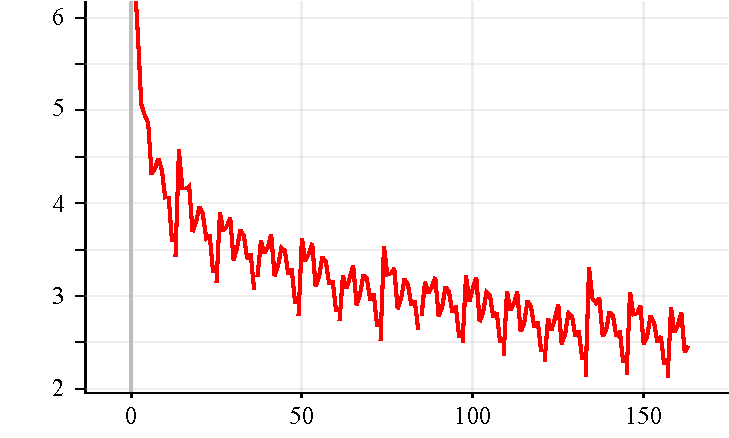
\includegraphics[width=.75\textwidth]{images/thesis/pretraining_loss}
\caption{Cross-entropy loss during the pre-training of \bart{-Base}.}
\label{fig:pretraining_loss}
\end{figure}

Additionally we record the cross-entropy loss on the evaluation data while fine-tuning
and report it in \autoref{fig:telco_finetuning_loss} for \telco{}
and in \autoref{fig:logsummary_finetuning_loss} for \logsummary{}.

\begin{figure}[htbp]
\centering
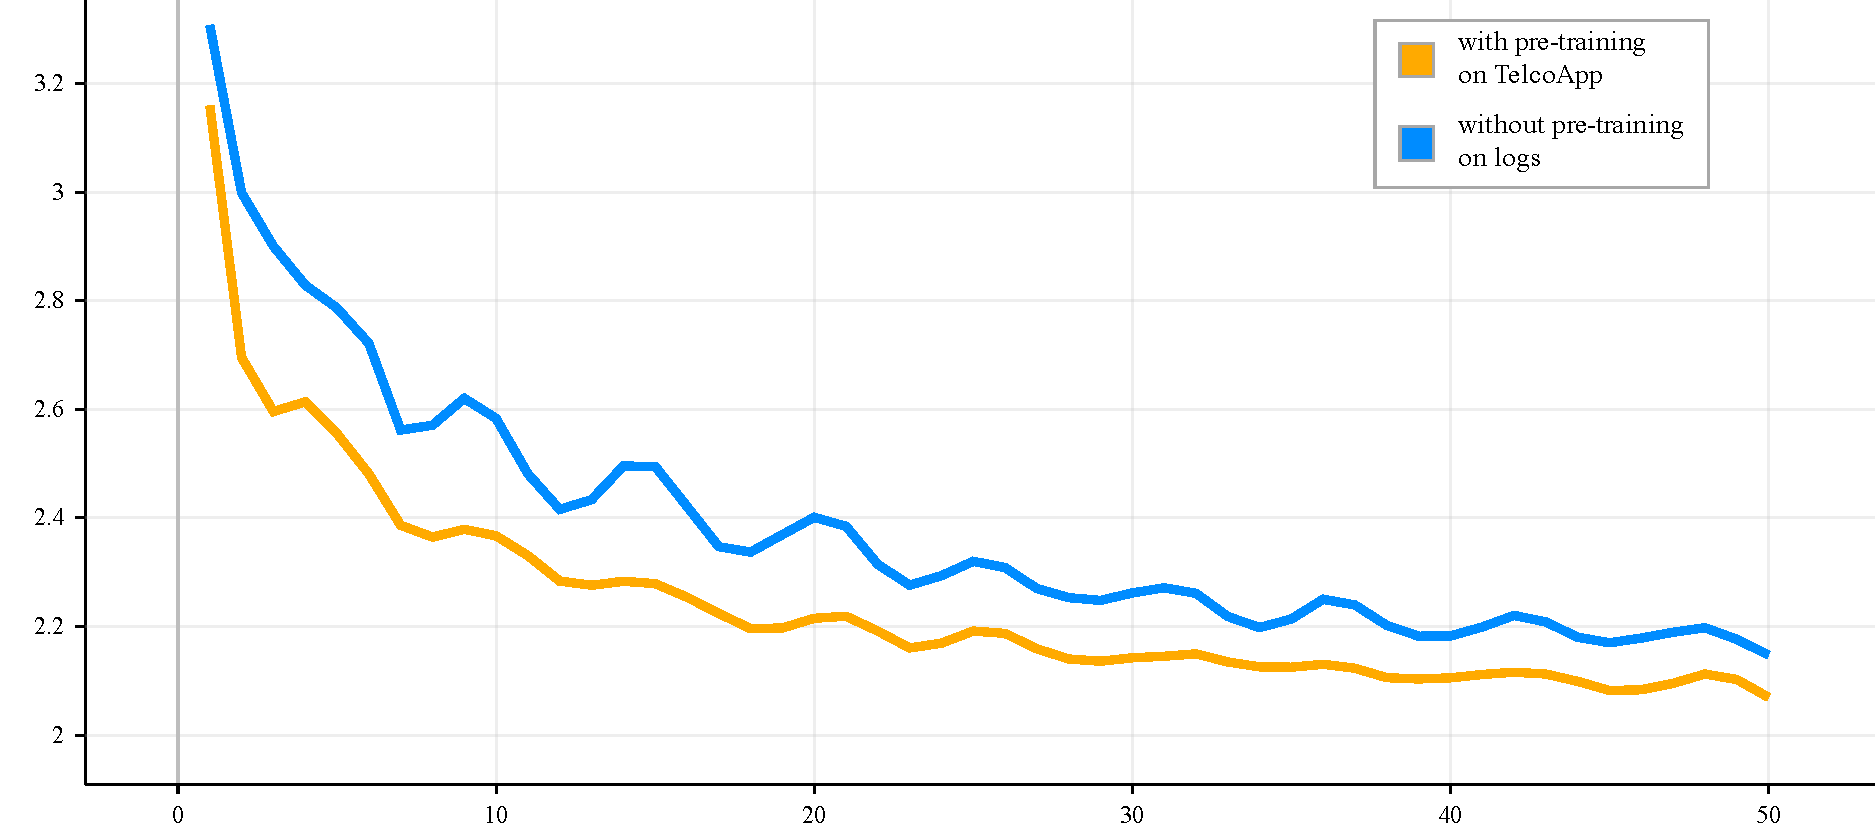
\includegraphics[width=.9\textwidth]{images/thesis/telcoapp_finetuning_loss}
\caption{Cross-entropy loss on the test set during the fine-tuning of \bart{-Base} and the variant pre-trained on \telco{}.}
\label{fig:telco_finetuning_loss}
\end{figure}

\begin{figure}[htbp]
\centering
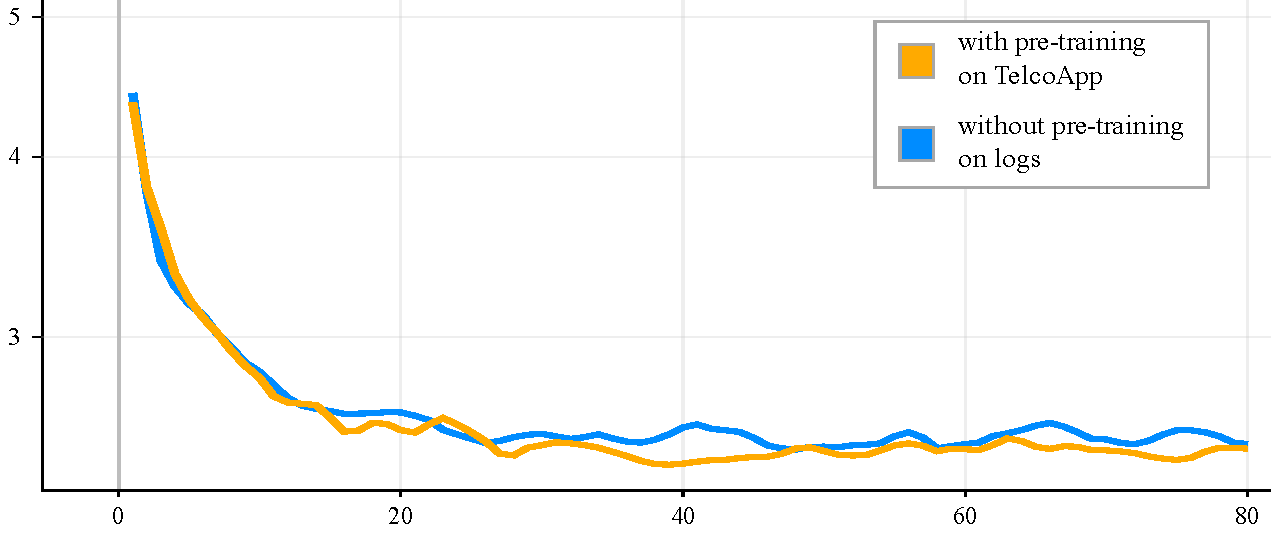
\includegraphics[width=.9\textwidth]{images/thesis/logsummary_finetuning_loss}
\caption{Cross-entropy loss on the test set during fine-tuning of \bart{-Base} and the variant pre-trained on \logsummary{}.}
\label{fig:logsummary_finetuning_loss}
\end{figure}

Finally, we present the results on the summarization datasets
in \autoref{tab:bart_pretrained_comparison_telco} for \telco{}
and in \autoref{tab:bart_pretrained_comparison_logsummary} for \logsummary{}.
The \(F_1\) scores of \acs*{rouge}-1, \acs*{rouge}-2 and sentence-level \acs*{rouge}-L are reported,
and the best results highlighted between the model that experienced further pre-training and the one that did not.
For comparison, we also include the results of \bart{-CNN} from \autoref{sec:evaluation_experiment_finetuned}.

\begin{table}[htbp]
\centering
\footnotesize
\begin{tabular}{lccc}
          & \multicolumn{3}{c}{\scriptsize{}\acs*{rouge}-1 / \acs*{rouge}-2 / \acs*{rouge}-LSent}\\
          & \h{\bart{-Base}}          & \h{\bart{-Base}}               & \h{\bart{-CNN}}\\
          & \scriptsize{}\h{not} pre-trained on log-data
          & \scriptsize{}further pre-trained on \h{\telco{}}
          & \scriptsize{}\h{not} pre-trained on log-data\\
\midrule
\acf{zsl} & 35.2/\h{26.3}/\h{29.2}    & \h{36.4}/25.4/26.1             & 39.2/31.1/33.3\\
\acf{fsl} & 39.4/31.5/35.8            & \h{39.9}/\h{32.1}/\h{35.9}     & 40.5/33.0/37.2\\
\end{tabular}
\caption{Mean \acs*{rouge} \(F_1\)-scores on \telco{} for the different BART variants.}
\label{tab:bart_pretrained_comparison_telco}
\end{table}

\begin{table}[htbp]
\centering
\footnotesize
\begin{tabular}{lccc}
          & \multicolumn{3}{c}{\scriptsize{}\acs*{rouge}-1 / \acs*{rouge}-2 / \acs*{rouge}-LSent}\\
          & \h{\bart{-Base}}          & \h{\bart{-Base}}               & \h{\bart{-CNN}}\\
          & \scriptsize{}\h{not} pre-trained on log-data
          & \scriptsize{}further pre-trained on \h{\telco{}}
          & \scriptsize{}\h{not} pre-trained on log-data\\
\midrule
\acf{zsl} & 25.6/13.8/23.6            & \h{26.8}/\h{14.4}/\h{24.3}     & 35.5/20.6/33.1\\
\acf{fsl} & 76.6/\h{66.4}/\h{71.1}    & \h{76.9}/66.3/70.3             & 76.9/65.9/69.9\\
\end{tabular}
\caption{Mean \acs*{rouge} \(F_1\)-scores of .}
\label{tab:bart_pretrained_comparison_logsummary}
\end{table}

We observe that pre-training alone does improve \ac{zsl} performance a bit,
at least in the \logsummary{} dataset,
but is simplify not enough to create a model able to produce meaningful summaries.
As the model has never been fine-tuned for summarization before, analogous to \bart{-Large},
this is to be expected.
The model has not yet learned that we expect it to write summaries.

All in all, the scores are quite similar after fine-tuning, even when compared to \bart{-CNN}.

\subsection{Discussion}

As can be seen in \autoref{fig:pretraining_loss} the \bart{-Base} model quickly adapts to the new pre-training data,
with the cross-entropy halving within the first 4 epochs.
By the time it reaches around 130 steps, the gains start to stagnate however.
To achieve further significant gains,
we believe it to be likely that the pre-training has to be scaled up to more steps (1000 - 10000).

Furthermore, the cross-entropy fluctuates considerably.
Whenever an epoch of pre-training is finished and a new one starts, the cross-entropy spikes.
This suggests that the log dataset is not homogeneous and the model partly forgets how to handle logs at the beginning of the dataset by the time it finishes an epoch.
The model still is able to consistently lower its cross-entropy overall,
but in the future one may want to shuffle the training data randomly to smooth out the pre-training process.

If we examine the performance of the pre-trained model in the summarization task on \telco{},
we notice that the continued pre-training indeed helped the model better predict the given data;
during fine-tuning it adapts more swiftly and maintains its head-start in cross-entropy even after the fine-tuning is finished.

Unfortunately, the positive impact of continued pre-training on cross-entropy remains confined to the \telco{} dataset.
On \logsummary{}, the pre-training in the domain of log-data did not help \bart{-Base} to make significant performance gains,
neither regarding perplexity nor the \acs*{rouge} metrics.
This is likely due to the difference in style, format and content of various log datasets.
Since \logsummary{} and \telco{} are diverse and distinct from one another,
the model was not able to transfer its newfound knowledge.

From the perspective of cross-entropy, the pre-training was successful for \telco{}.
This improvement in cross-entropy and perplexity however does not translate in a significant difference in summarization performance:
Both the \ac{prefsl} model and the \ac{fsl} baseline show near identical \acs*{rouge}-scores.

Ultimately, continued pre-training did not deliver on the performance improvements we initially expected from it.
We speculate that continued pre-training can still be useful for other tasks than the ones we studied
because the model was able to achieve lower perplexity much faster, even if pre-training did not help on our datasets.

Last but not least,
we remark that after fine-tuning, the base model achieved similar performances compared to the \bart{-CNN} model on both datasets.
To us, this indicates not only that previous training in another summarization dataset is not that relevant to our application
but also that smaller models may be able to achieve similar performances to variants with more parameters.
Since smaller models consume less memory and are faster, both during training and text generation, this is a promising result.

\section{Comparison with the LogSummary framework}\label{sec:evaluation_experiment_logsummary}

Besides introducing a dataset of summarized log-data,
\citeauthor*{log_summary} also introduced their own framework for summarizing logs called \emph{LogSummary}~\parencite{log_summary},
which is explained in greater detail in \autoref{ch:related_work}.

In this section, we aim to compare our results directly with this previous work.
As the LogSummary framework is specifically laid out to only extract parts of any given log messages,
it would perform badly on the two summarization datasets \hadoop{} and \telco{} we introduced ourselves,
where models are expected to reproduce entire log messages.
Therefore we only compare on the \logsummary{} dataset, however we will differentiate between each subdataset as was done in \parencite{log_summary}.

\subsection{Experimental Setup}

We choose our best performing model (\bart{-CNN}) and compare it with the LogSummary framework.

To keep the comparison fair, we need to skip our simplification step from \autoref{subsec:preprocessing},
as the framework works directly on the log messages without needing any simplification.
As such, we take the baseline \bart{-CNN} and fine-tune it on the raw log messages,
otherwise using the same \ac{fsl} setting as in the previous experiment.
To find an optimal length penalty for the beam-search, we again employ an automatic hyperparameter search with 20 trials.\\
We take this as an opportunity to test how helpful our simplification step was for the model,
by comparing the results with the \bart{-CNN} model fine-tuned on the simplified messages.

For the LogSummary framework, we use the results as reported in \parencite{log_summary}.
For the two datasets (Spark and Zookeeper) not included in the original article,
we manually run the LogSummary framework on these datasets and fix any errors encountered.%
\footnote{LogSummary's repository is available at: \url{https://github.com/WeibinMeng/LogSummary}}
This also requires us to manually train two Log2Vec~\parencite{log2vec} models, which are used by the LogSummary framework.%
\footnote{Log2Vec's repository is available at: \url{https://github.com/NetManAIOps/Log2Vec}}
As we could not find any specific information on the amount of data used to train the Log2Vec models in \parencite{log_summary},
we decide to use the \verb+2k.log+-files provided by \parencite{loghub} for the respective datasets,
as this is also the example data used in the Log2Vec repository.

To verify we conducted this process correctly,
we evaluate the LogSummary framework on the HDFS dataset using their pipeline
and receive mean \acs*{rouge}-1 scores of \(54.7\), \(72.1\) and \(45.4\) for \(F_1\), precision and recall respectively.
For the BGL dataset we obtain \(77.4\), \(83.0\) and \(76.1\).
While these do differ from the scores reported in \parencite{log_summary},
they do so only by a small margin of 1 to 5 points.
Therefore we assume we executed the LogSummary framework correctly and proceed to evaluate it on the two new datasets.

For this experiment only, we use a different implementation of the \acs*{rouge} metric, namely the one used by the LogSummary framework%
\footnote{That implementation is available at \url{https://github.com/pltrdy/rouge}.}, to keep the comparison fair.

\subsection{Results}

Following \parencite{log_summary}, we primarily investigate values of the \acs*{rouge}-1 metric:
The reasoning for comparing only the \acs*{rouge}-1 values provided by \citeauthor*{log_summary}
is that the different authors of each reference summary may have written words and phrases in different succession,
ranking extracted segments by different priorities.
The results are shown in \autoref{tab:comparison_rouge1_logsummary} with the best results on each subdataset highlighted.

The results for the LogSummary framework are for the whole dataset,
while the results of our model are calculated on the test set only.
Since 95 out of 100 examples in each subdataset are in the test set,
the results should still be comparable.

\begin{table}[htbp]
\centering
\footnotesize
\begin{threeparttable}
\begin{tabular}{l@{\qquad}c@{\qquad}c}
                    & \multicolumn{2}{c}{\scriptsize{}\(F_1\) / precision / recall}\\
                    & \h{LogSummary framework}            & \h{\bart{-CNN} \acs{fsl}} (ours)\\
\midrule
BGL                 & \h{72.5}/\h{81.5}/70.3\tnote{*}     & 71.9/72.8/\h{75.3}\\
HDFS                & 53.8/75.9/43.2\tnote{*}             & \h{77.2}/\h{80.2}/\h{75.5}\\
HPC                 & 84.0/81.9/\h{91.1}\tnote{*}         & \h{84.2}/\h{82.8}/88.5\\
Proxifier           & 86.4/87.9/85.7\tnote{*}             & \h{93.1}/\h{99.1}/\h{89.8}\\
Spark               & 59.4/68.9/53.1\tnote{\(\dagger\)}   & \h{79.5}/\h{78.2}/\h{83.8}\\
Zookeeper           & 50.7/58.9/46.0\tnote{\(\dagger\)}   & \h{74.1}/\h{73.6}/\h{79.5}\\
\midrule
average             & 67.8/75.8/64.9                      & \h{80.0}/\h{81.1}/\h{82.1}\\
\bottomrule
\end{tabular}
\begin{tablenotes}
\item[*] Scores as reported by \parencite{log_summary}.
\item[\(\dagger\)] Scores as identified by us from running the framework manually.
\end{tablenotes}
\caption{Mean \acs*{rouge}-\(1\) \(F_1\), precision and recall on the subdatasets of \logsummary{}.}
\label{tab:comparison_rouge1_logsummary}
\end{threeparttable}
\end{table}

We also report the sentence-level \acs*{rouge}-L scores for our approach:
In \autoref{tab:comparison_preprocessing_logsummary} we display the performance of our \bart{-CNN} model on each subdataset of \logsummary{},
and provide the results of the \bart{-CNN} fine-tuned on the simplified messages from \autoref{sec:evaluation_experiment_finetuned} for comparison.

Sentence-level \acs*{rouge}-L provides a measure to evaluate how much information overlap there is between the model generated summary and human-written references,
additionally estimating the model's ability to preserve the order of extracted segments.
Thus we can also assess how well the model can prioritize segments from the subjective ordering assigned to them by the authors of the summaries.

\begin{table}[htbp]
\centering
\footnotesize
\begin{tabular}{l@{\qquad}c@{\qquad}c}
                    & \multicolumn{2}{c}{\scriptsize{}\(F_1\) / precision / recall}\\
                    & \h{simplified messages} & \h{regular messages}\\
\midrule
BGL                 & 59.0/51.8/\h{76.9}      & \h{67.8}/\h{68.4}/71.3\\
HDFS                & 69.3/67.6/\h{73.3}      & \h{69.4}/\h{71.9}/67.9\\
HPC                 & 75.6/71.7/\h{86.0}      & \h{81.1}/\h{79.7}/85.4\\
Proxifier           & \h{95.0}/97.8/\h{93.2}  & 92.2/\h{98.0}/89.1\\
Spark               & \h{68.3}/64.5/\h{75.8}  & 67.0/\h{65.9}/70.5\\
Zookeeper           & \h{62.7}/60.0/\h{68.6}  & 61.5/\h{61.0}/66.3\\
\midrule
average             & 71.6/68.9/\h{79.0}      & \h{73.1}/\h{74.1}/75.1\\
\bottomrule
\end{tabular}
\caption{Mean sentence-level \acs*{rouge}-\(L\) \(F_1\), precision and recall of the fine-tuned \bart{-CNN} models on the subdatasets of \logsummary{}.}
\label{tab:comparison_preprocessing_logsummary}
\end{table}

\subsection{Discussion}

\paragraph{Evaluation of our text simplification during preprocessing}

First, we briefly examine how \bart{-CNN} handles the log-data without using our simplifications;
To our surprise the model performs well, even surpassing the average performance of our previous \bart{-CNN} model using the simplified messages.
The model operating on the raw messages manages to achieve higher precision, only slightly falling of on recall.

However, any direct comparisons should be taken with a grain of salt:
The length penalty the hyperparameter search found for \bart{-CNN} operating on the raw messages encourages shorter summaries than the one for the previous model,
likely being a major cause in the precision/recall-tradeoff we observe.

Still, on the HPC dataset both models achieve almost the same recall, but the model operating on raw messages is more precise.
At the very least, this indicates that there are situations where our simplification step is not helpful.
Further still, at least on the \logsummary{} dataset, the simplification step is likely not a major factor in increasing a model's performance:
After further fine-tuning, \bart{-CNN} is able to summarize raw log messages well enough.

While this means that our simplification step may have been unnecessary,
the possibility that pre-trained \ac{nlp} models may not require a simplification step
based on error-prone regular expressions is actually very promising.

The necessity of simplification may change on datasets including more complex patterns;
we believe it to be likely that simplifying long patterns is still important,
like java stack traces or long file-paths present in the \hadoop{} and \telco{} datasets.
These passages are especially long and contain little important information, displacing more important context.
Altogether though, our simplification step can likely be scaled down without negatively impacting model performance.

\paragraph{Comparison with previous work}

In general, the \bart{-CNN} fine-tuned on raw messages performs comparatively well.
On the BGL dataset, the \(F_1\)-scores are similar, but the summarization framework is more precise.
The contrary is true on the HPC dataset, where \bart{-CNN} is more precise.
On all other remaining datasets, \bart{-CNN} strictly outperforms the previous work by at least \(7\) points regarding the \(F_1\) measure.
Overall, we achieve improved \acs*{rouge}-1 \(F_1\) scores of \(12\) points on average.

Of course, risk of overfitting is present when using deep learning methods.
As the LogSummary framework makes use of unsupervised learning algorithms, it is not affected by this problem.
However, the vocabulary overlap of summaries between training data and test data
is the lowest for the \logsummary{} dataset across all studied datasets
(see \autoref{tab:training_test_vocab_overlap} on \autopageref{tab:training_test_vocab_overlap}).
We do not believe the improved performance of \bart{-CNN} can be explained solely on the basis of overfitting.

Still, we previously only reported the overall vocabulary overlap of summaries,
but there may be substantial differences between the subdatasets of \logsummary{}.
Thus we also report the overlap for each subdataset in \autoref{tab:logsummary_subdatasets_vocab_overlap}.

\begin{table}[htbp]
\centering
\footnotesize
\begin{tabular}{cccccc}
BGL                                 & HDFS                         & HPC &
Proxifier                           & Spark                        & ZooKeeper\\
\midrule
\(\frac{17}{139} \approx 12.230\%\) & \(\frac{10}{25} = 40.000\%\) & \(\frac{26}{66} \approx 39.394\%\) &
\(\frac{17}{22}  \approx 77.273\%\) & \(\frac{20}{61} = 32.787\%\) & \(\frac{22}{72} \approx 30.556\%\)
\end{tabular}
\caption{Ratio of words common between summaries in the respective training and test sets for all subdatasets of \logsummary{}.}
\label{tab:logsummary_subdatasets_vocab_overlap}
\end{table}

Here we see a more diverse picture:
The BGL dataset certainly brings down the average vocabulary overlap between training and test set.
As the summaries on HDFS and Proxifier are less varied in their vocabulary, both in relative and absolute terms,
it is possible that \bart{-CNN} overfits on these datasets.
However, the same model still performs well on the other more diverse datasets,
showing that it is capable of applying its knowledge even on inputs different from its training data.

As opposed to the LogSummary framework, which required a separate Log2Vec model for each subdataset to achieve peak performance,
we trained \bart{-CNN} on all six datasets simultaneously.
Our results suggest that \bart{-CNN} is applicable even in situations
where logs are generated from heterogeneous subsystems with different logging styles.

Last but not least, if we compare \acs*{rouge}-1 to the sentence-level \acs*{rouge}-L for \bart{-CNN},
we observe that the reduction in recall and precision is not drastic, both falling by only 7 points.
This means that \bart{-CNN} was able to mostly imitate the style and subjective structure of the human-written summaries.
We speculate the model can thus also be adapted to other extractive summary styles wished for in practical applications.

All in all, we showed that pre-trained \ac{nlp} models can effectively summarize the contents of log-data,
even with minimal fine-tuning required.
As a \ac{seq2seq} architecture \bart{-CNN} not only outperforms previous work, but is also more flexible by design.

\section{Threats to Validity}\label{sec:threats_to_validity}

As a conclusion to this chapter, we discuss some aspects regarding the validity of our results and conclusions.

\paragraph{Sensitivity to hyperparameters}

The hyperparameters of the beam-search greatly influence the performance of our models.
Previous research confirms this finding,
as \citeauthor*{solving_length_problem} show that machine translation systems are sensitive to the length penalty used
and that different tasks and datasets require different penalties~\parencite[9]{solving_length_problem}.

Finding optimal values is challenging;
The differences observed between the transformer models in our experiments
could in part be caused by suboptimal values for these generation parameters.
We tried to mitigate this in our experiments by using automatic hyperparameter searches
and consulting multiple perspectives (including examining perplexity, which is unaffected by these parameters) to select the best-performing models.
Yet, we cannot fully exclude that some of our findings are influenced by suboptimal hyperparameters,
especially when the differences between performances is small, as was the case for the BART variants in \autoref{sec:evaluation_experiment_finetuned}
or when we examined the effects of pre-training in \autoref{sec:evaluation_experiment_pretraining}.

\paragraph{Problems of \acs*{rouge} as a measure of quality}

Ever since the publication of the \acs*{rouge} metrics, several shortcomings have been pointed out by the academic community:
\begin{itemize}
\item \Acs*{rouge} is unaware of synonyms and expects summaries to closely match the reference summaries~\parencite{rouge2}.
\item In general, \acs*{rouge} only judges the overlap in vocabulary and longer text segments,
      but cannot judge fluency and factual consistency.
      These qualities need to be judged separately, for instance during trials with human judges~\parencite[546]{summarization_critical_evaluation}.
\item Surveys with human judges suggest \acs*{rouge} may be better fit for evaluating extractive models than abstractive models.
      For past model architectures \citeauthor*{summarization_critical_evaluation}
      investigated the correlation of \acs*{rouge}-scores to human judgments of quality:\\
      When considering extractive summaries only, \acs*{rouge}-scores were moderately correlated to human judgments of relevance, fluency, comprehensibility and factual coherence;
      such correlations remain less clear-cut for abstractive summaries~\parencite[545-546]{summarization_critical_evaluation}.
\end{itemize}

Since abstractive models create novel text sequences,
they may have a higher tendency to introduce factual inconsistencies~\parencite[546]{summarization_critical_evaluation},
which \acs*{rouge} cannot judge.
However, from manual inspection of the generated summaries,
we generally observe that the summaries closely follow an extractive style in our case,
not including novel sequences of words.
As our datasets are purely extractive, they encourage this behavior.

We believe this to be beneficial to the applicability of \acs*{rouge} to measure the quality of summaries on our datasets,
since many of the problems described above are directed towards comparing texts that are syntactically different,
but have the same semantic contents.
As both the generated summaries and the reference summaries closely follow the style of the inputs, this should be less of a concern.

\paragraph{Biases in logs}

In the past, summarization models trained on news articles showed a significant bias for the first three sentences of an article.
This has been attributed to a layout bias in journalism where the first parts of an article usually contain more important information~\parencite[544-546]{summarization_critical_evaluation}.
Thus \emph{Lead-3}, selecting the first three sentences of an article, performs well as a heuristical summary for news articles.

Lead-3 as a heuristic has next to no meaning in the context of log-data,
because messages in logs roughly follow a chronological order and are not ordered by significance.
However, there may be other biases in the data that could be used influence performance and should be accounted for.
A few examples come to mind:
\begin{itemize}
\item The setup operations executed at the startup of a system are likely to produce less important log-entries.
      If a model received only inputs that started at the beginning of a log,
      it may learn to ignore the first share of its input.

      On the \hadoop{} dataset it is the case that some of the model inputs start at the beginning of a log,
      where the startup operations happen,
      however the dataset also contains many input documents that start at other portions of a log.
\item Similarly, due to the way we selected the relevant portions of log-data we use as inputs on the \telco{} dataset,
      some of the model inputs necessarily start with log messages that are deemed important by the summarization task based on common log events.
      In these cases it may be advisable to perturb the inputs by including additional log messages at the beginning.
\item Each logging system may exhibit their own biases, with certain formats representing more important messages.
      Consider for example messages starting with \texttt{Diagnostics report from attempt} in the \hadoop{} dataset.
      As we saw in \autoref{tab:bart_cnn_hadoop_disk_full_example} on \autopageref{tab:bart_cnn_hadoop_disk_full_example} these usually represent anomalous messages,
      but not in all cases.
      Operators may find such messages useful in order to identify problems, but they may facilitate overfitting \ac{nlp} models.
\item While there are many lists of \emph{stop words}, which represent words that are less likely to convey important semantic information,
      it is unclear if these apply well to application logs.%
      \footnote{See \url{https://github.com/igorbrigadir/stopwords} for an overview of different stop word lists.}
      Words present in stop word lists are often ignored when evaluating a model using a metric.
      For example, \acs*{rouge} can optionally omit such words when evaluating the quality of a summary.
\item Log-entries often contain metadata such as severity-levels (error, debug, \ldots).
      We suspect errors and warnings may contain a significantly greater share of important information than the average log-entry.
      Related to this assumption, in the past system maintainers used basic keyword searches
      (e.g. searching for words like \emph{failure} or \emph{warning})
      to identify problematic log-lines~\parencite[307-308]{not_basic_keyword_search}.
\item Another potentially important metadata is the software component where the log message originated from.
      Some components will produce more important messages than others,
      because they play different roles in the operation of the system.
      It is possible that components issuing few messages are more likely to write important messages,
      because they represent software execution paths seldomly followed.
\end{itemize}
To avoid such biases and improve their generality, our models did not receive any metadata as inputs.
Still, our models could still be susceptible to the other biases mentioned and further biases not considered in these examples.

On the whole, biases present in log-data are not well researched, even though they are an important aspect influencing the performance and generality of models.
In other summarization datasets, like CNN/DailyMail and XSum, such biases are well-researched and accounted for during the design and evaluation of a model.
Consider for instance the removal of duplicated trigrams employed by BART on the CNN/DailyMail dataset,
which past research has shown to be beneficial~\parencites{bart}{beam_search_duplicate_ngram_removal}:
In other summarization datasets that contain repetitions (like BigPatent~\parencite{bigpatent}) this may be detrimental to the model's performance,
but it is actually helpful here.

\paragraph{Threat to universality}

One actuality we frequently observed during our experiments is that logs can be quite diverse:
\begin{itemize}
\item Logs originating from different systems may use dissimilar vocabularies
      and show less overlap than other previously researched summarization domains.
      As can be seen in \autoref{fig:datasets_vocab_overlap} on \autopageref{fig:datasets_vocab_overlap},
      the datasets from the news domain show a much larger overlap in frequently used words than logs do.
      Further still, logs share little vocabulary with common summarization datasets in general.
\item Logs vary in degree of correct use of capitalization and punctuation,
      meaning that there is no perfect choice for a separator between log messages concerning the pre-trained models investigated.
\item As seen in \autoref{tab:logsummary_subdatasets_vocab_overlap} on \autoref{tab:logsummary_subdatasets_vocab_overlap},
      even by randomly sampling only 5 out of 100 examples for training,
      one can get widely different overlaps in vocabulary for training and test sets,
      on logs originating from different systems.
      Some systems show multifaceted use of different words, while others consist of only a few different log events,
      making it easy to accidentally overfit models on these datasets.
\item Different summarization tasks are applicable to different log datasets.
      We presented the conditions in which we believe our summarization tasks to identify meaningful log events,
      that can be used as the basis for reference summaries,
      yet the nature of the resulting summaries is quite different.
      Summaries based on \emph{common log events} are by nature quite homogeneous when only considering a single root cause,
      while summaries based on \emph{non-normal log events} can be more diverse.

      Both our proposed summarization tasks are \emph{failure-oriented},
      as they require a failure to be present to be applicable,
      but they make use of different assumptions inspired from the log datasets they were applied on.
\item Even logs originating from the same system can be very different,
      as we observed on the \hadoop{} dataset:
      During some failures a group of message is periodically written to the log, leading to large log files,
      which consist of mostly redundant information.
      Other failures only produce small amounts of more diverse anomalous messages, reducing the overall redundancy of the log.
\end{itemize}
This diversity is part of what makes summarization on log-data challenging.
Even worse, it means that our models and summarization tasks may not be applicable to logs from other systems.

\emph{Log summarization} cannot be understood as a singular task,
rather requirements for summaries will vary from system to system.
Even for the human-written summaries in \logsummary{} which all follow a similar style,
the model's performance varies between log segments from different systems.
Our findings may not apply to other log datasets.

In practice, this means that a model should be fine-tuned on each specific dataset it is used on in order to achieve peak performance.
Thankfully,
tuning a pre-trained transformer model with only a few examples can be enough to improve performance and achieve useful results,
as we have demonstrated in our experiments.
Additionally, a single model may be able to handle logs from heterogeneous systems, as our results in the \logsummary{} dataset suggest.

\paragraph{Lack of user studies}

As the idea of textual log summarization is relatively young,
none of the datasets we employ have previously been studied in the context of a user study.
While \citeauthor*{log_analysis} previously found that presenting a condensed representation of log-data to users
can greatly speed up their ability to analyze said data~\parencite{log_analysis},
it is not possible for us to determine if the same is true for the summaries studied by us.

On the \logsummary{} dataset, the summaries are human-written, implying at least a basic degree of quality.
However, on the other two datasets we employed our own summarization tasks,
which construct reference summaries using semi-automatic means.
While we presented several arguments why we believe our summarization tasks to produce informative summaries,
it is still unclear whether system experts would find the resulting reference summaries valuable.
